\documentclass{article}

\usepackage{PRIMEarxiv}

\usepackage{hyperref}
\usepackage{url}
\usepackage{booktabs} % professional-quality tables
\usepackage[utf8]{inputenc} % allow utf-8 input
\usepackage[T1]{fontenc}    % use 8-bit T1 fonts
\usepackage{microtype}
\usepackage{fancyhdr}
\usepackage[style=apa]{biblatex}
\addbibresource{references.bib} % Link to your .bib file
%\usepackage[margin=1in]{geometry} % Removed to avoid option clash
\usepackage{graphicx} % For including images
\usepackage{rotating}

\makeatletter
\renewbibmacro*{cite:author}{%
  \iffieldequals{namehash}{\cbx@lasthash}
% Multiple cites in one command
   {\setunit{\compcitedelim}%
    \printtext[bibhyperref]{%
      \usebibmacro{cite:plabelyear+extradate}}}%
% Single cite
   {\printtext[bibhyperref]{%
      \ifnameundef{labelname}
% No author/editor
       {\usebibmacro{cite:noname}%
         \savefield{namehash}{\cbx@lasthash}}
% Normal cite
       {\ifnameundef{shortauthor}
         {\printnames{labelname}}%
         {\cbx@apa@ifnamesaved
            {\printnames{shortauthor}}
            {\printnames[labelname]{author}%
             \addspace\printnames[sabrackets]{shortauthor}}}%
          \savefield{namehash}{\cbx@lasthash}}}}%
   \setunit{\multicitedelim}}

\renewbibmacro*{cite}{%
  \iffieldequals{namehash}{\cbx@lasthash}
% Multiple cites in one command
   {\setunit{\compcitedelim}%
    \printtext[bibhyperref]{%
      \usebibmacro{cite:plabelyear+extradate}}}%
% Single cite
   {\printtext[bibhyperref]{%
      \ifnameundef{labelname}
% No author/editor
       {\usebibmacro{cite:noname}%
         \setunit{\printdelim{nameyeardelim}}%
         \usebibmacro{cite:plabelyear+extradate}%
         \savefield{namehash}{\cbx@lasthash}}
% Normal cite
       {\ifnameundef{shortauthor}
         {\printnames{labelname}}%
         {\cbx@apa@ifnamesaved
           {\printnames{shortauthor}}
           {\printnames[labelname]{author}%
            \addspace\printnames[sabrackets]{shortauthor}}}%
         \setunit{\printdelim{nameyeardelim}}%
        \usebibmacro{cite:plabelyear+extradate}%
        \savefield{namehash}{\cbx@lasthash}}}}%
   \setunit{\multicitedelim}}

\renewbibmacro*{textcite}{%
  \iffieldequals{namehash}{\cbx@lasthash}
% Compact cite - more than one thing for same author
    {\setunit{\compcitedelim}%
     \printtext[bibhyperref]{%
       \usebibmacro{cite:plabelyear+extradate}}}
% New cite
    {\ifbool{cbx:parens}
       {\bibcloseparen\global\boolfalse{cbx:parens}}
       {}%
     \setunit{\textcitedelim}%
     \ifnameundef{labelname}
     % No author/editor
       {\iffieldundef{shorthand}%
    % Cite using title
         {\printtext[bibhyperref]{\usebibmacro{cite:noname}}%
          \setunit{\global\booltrue{cbx:parens}%
                   \printdelim{nonameyeardelim}%
                   \bibopenparen}%
          \printtext[bibhyperref]{%
            \usebibmacro{cite:plabelyear+extradate}}}
    % Cite using shorthand
         {\printtext[bibhyperref]{%
            \usebibmacro{cite:shorthand}}}}
  % Normal cite with author/editor
  % Normal full cite
       {\printtext[bibhyperref]{%
          \ifnameundef{shortauthor}%
    % Normal full cite
           {\printnames{labelname}}
    % Cite using short author
           {\cbx@apa@ifnamesaved
             {\printnames{shortauthor}}
             {\printnames[labelname]{author}}}}%
  % Year
        \setunit{\global\booltrue{cbx:parens}%
                 \printdelim{nameyeardelim}%
                 \bibopenparen}%
  % Put the shortauthor inside the year brackets if necessary
        \printtext[bibhyperref]{%
          \ifnameundef{shortauthor}
           {}
           {\cbx@apa@ifnamesaved
             {}
             {\printnames{shortauthor}%
              \setunit{\printdelim{innernameyeardelim}}}}%
  % Print prenote (belongs to first cite)
        \ifnumequal{\value{citecount}}{1}
           {\usebibmacro{prenote}}
           {}%
  % Actual year printing
        \usebibmacro{cite:plabelyear+extradate}%
  % Save name hash for checks later
        \savefield{namehash}{\cbx@lasthash}}%
    \stepcounter{textcitecount}}}}

\renewbibmacro*{cite:plabelyear+extradate}{%
  \iffieldundef{labelyear}{}
    {\clearfield{labelmonth}% don't want months in citations
     \clearfield{labelday}% don't want days in citations
     \clearfield{labelendmonth}% don't want months in citations
     \clearfield{labelendday}% don't want days in citations
     \clearfield{labelyeardivision}% don't want yeardivisions in citations
     \clearfield{labelendyeardivision}% don't want yeardivisions in citations
     \iffieldsequal{labelyear}{labelendyear}% Don't want no-op year ranges
       {\clearfield{labelendyear}}
       {}%
     \iffieldundef{origyear}
       {}
       {\printorigdate%
        \setunit*{\addslash}}%
     \iffieldundef{related}
       {}
       {\iffieldequalstr{relatedtype}{reprintfrom}
         {\entrydata*{\thefield{related}}{\printlabeldateextra}%
          \setunit*{\addslash}}
         {}}%
     \printlabeldateextra}}

\renewbibmacro*{citeyear}{%
  \iffieldundef{labelyear}
    {\usebibmacro{cite:init}}
    {\iffieldequals{namehash}{\cbx@lasthash}
       {\setunit{\compcitedelim}%
        \printtext[bibhyperref]{\usebibmacro{cite:plabelyear+extradate}}}
       {\printtext[bibhyperref]{\usebibmacro{cite:plabelyear+extradate}}%
        \savefield{namehash}{\cbx@lasthash}}}%
  \setunit{\multicitedelim}}
\makeatother

%Header
\pagestyle{fancy}
\thispagestyle{empty}
\rhead{ \textit{ }} 

% Update your Headers here
\fancyhead[LO]{Harnessing AI and Language Models for Predictive Modeling of Patient Health Deterioration}

%% Title
\title{Harnessing AI and Language Models for Predictive Modeling of Patient Health Deterioration}

\author{
  Khor Kean Teng \\
  WQD 7005 Data Mining \\
  Faculty of Computer Science \& Information Technology, University Malaya \\
  Kuala Lumpur\\
  \texttt{\{u2004763\}@siswa.um.edu.my} \\
}

\begin{document}

\maketitle

\begin{abstract}
  This report details a project aimed at leveraging Artificial Intelligence (AI), including Large Language Models (LLMs), Smaller Language Models (SLMs), and Generative AI (GenAI), to predict patient health deterioration. The core objective was to explore the efficacy of these advanced technologies in a healthcare context, specifically through the simulation of patient vital signs and questionnaire data, and the subsequent development of predictive models. Key methods employed include dataset simulation using GenAI (\textit{Gemini 2.5 Flash-Preview-0417}), feature engineering from textual data via LLMs/SLMs (\textit{BioBERT, Gemini 2.5 Flash-Preview-0417}), development of both traditional machine learning (\textit{Random Forest, XGBoost, Neural Networks}) and transformer-based tabular models (\textit{TabTransformer, FT Transformer}) for deterioration prediction, and specialized Natural Language Processing (NLP) tasks such as sentiment analysis (\textit{Google BERT-Large}), clinical Named Entity Recognition (\textit{Bio-Clinical BERT}), and questionnaire response classification (\textit{BERT-base}). The main findings highlight the comparative performance of these diverse models, demonstrating strong predictive capabilities, particularly from the FT Transformer in patient deterioration and BERT-based models in NLP tasks. The effectiveness of AI in interpreting complex model outputs (using \textit{Gemini 2.5 Flash-Thinking-Preview-0417, Grok 3, Gemini 2.5 Flash-Thinking-Preview-0520}) was also a significant outcome. This work underscores the potential of advanced AI in enhancing predictive healthcare analytics and provides recommendations for future model refinement, data enhancement, and ethical deployment.
\end{abstract}

% keywords can be removed
\keywords{: BERT \and Transformer \and Artificial Intelligence \and Generative AI \and Small Language Models (SLMs)}

\section{Introduction}

This academic report details an investigation into leveraging Artificial Intelligence (AI) for the early prediction of patient health deterioration, a critical aspect of modern healthcare aimed at improving outcomes, optimizing resource allocation, and reducing costs. Traditional monitoring often fails to capture subtle early decline, whereas AI, particularly Large Language Models (LLMs), Smaller Language Models (SLMs), and Generative AI (GenAI), offers transformative potential for continuous, proactive analysis of complex patient data. These models excel at understanding unstructured text like clinical notes (LLMs/SLMs) and generating synthetic datasets for research where real-world data is limited (GenAI). The primary objective of this project was to harness these AI capabilities for predictive modeling of patient deterioration. This was achieved by simulating a comprehensive patient dataset using GenAI, engineering relevant features from structured and unstructured data (including medical history and questionnaire responses via LLMs/SLMs), developing and evaluating machine learning and deep learning models for deterioration prediction, performing specialized NLP tasks for deeper textual insights, and utilizing AI to interpret complex model results. The scope of work thus encompassed dataset simulation, feature engineering, predictive modeling, thorough model evaluation, and AI-assisted reporting. This report is structured to first detail the methodology for these tasks (\textit{Section 2}), then present and discuss the results from classification and NLP tasks, including AI-assisted interpretations (\textit{Section 3}). Subsequently, \textit{Section 4} concludes with key findings and objective achievement, \textit{Section 5} offers recommendations for future work, and \textit{Section 6} discloses the AI tools and techniques employed.
\section{Methodology}

\begin{sidewaysfigure}[p]
    \centering
    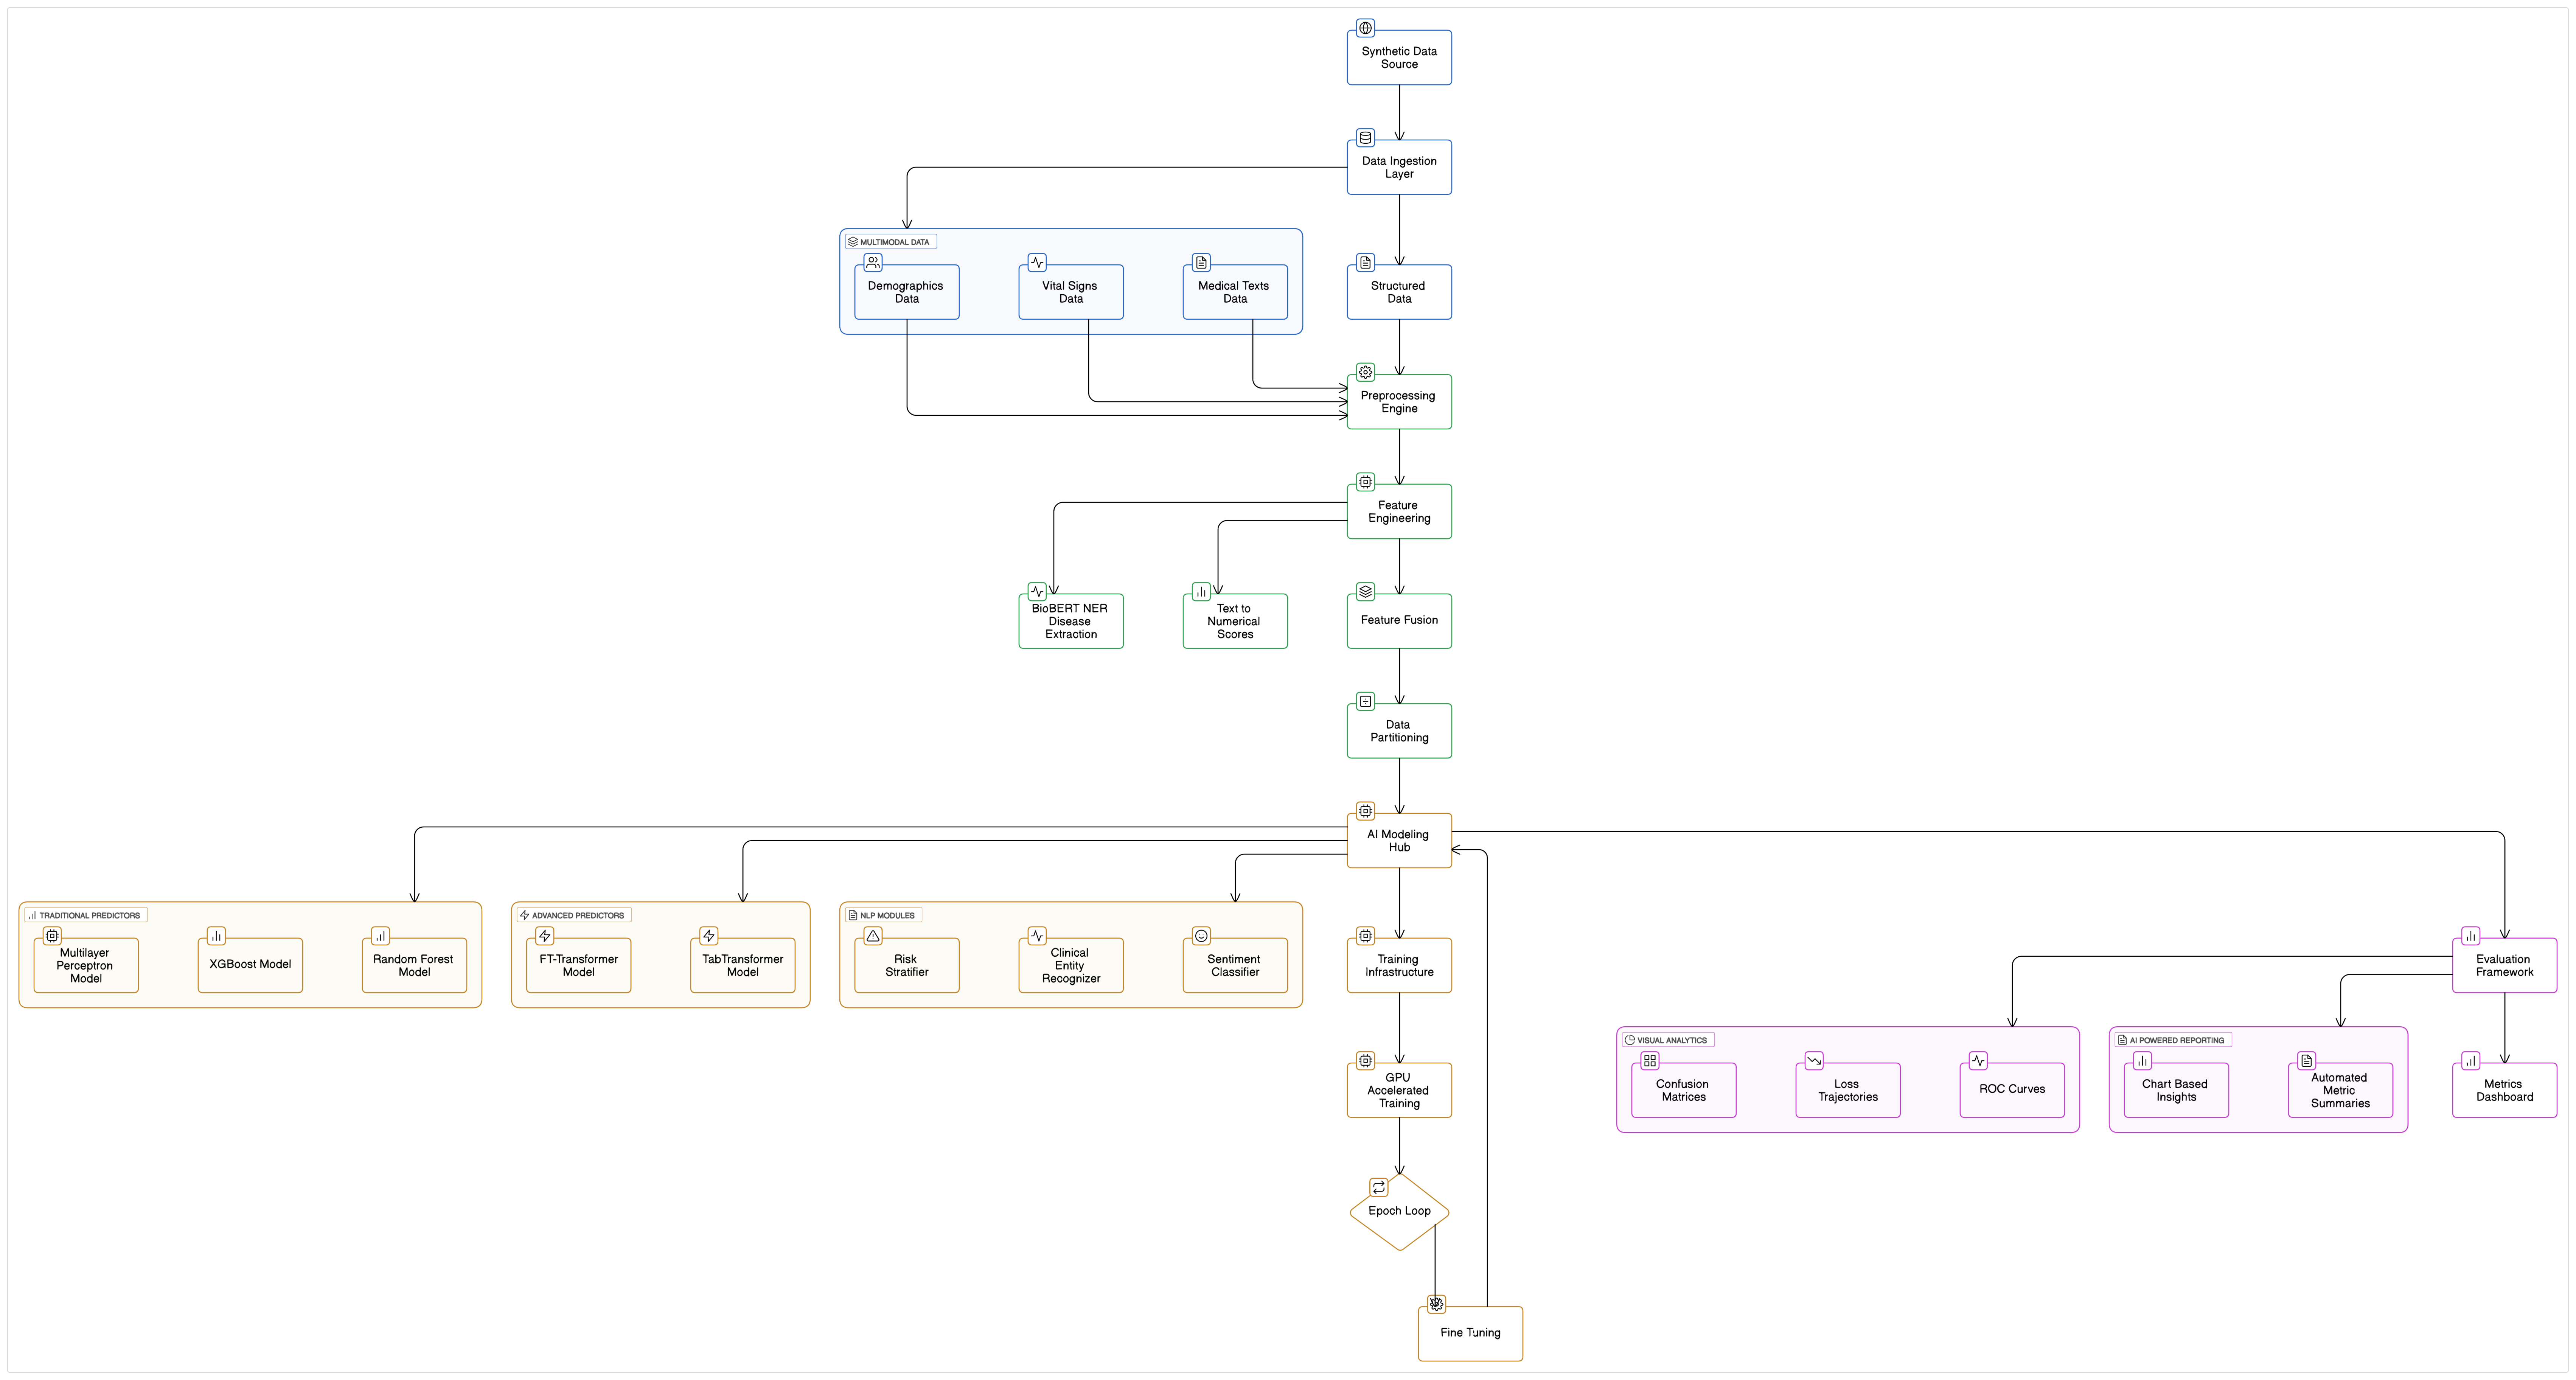
\includegraphics[width=0.8\textwidth]{../images/architecture.png} % Replace with your image path
    \caption{Project Architecture Overview}
    \label{fig:project_architecture}
\end{sidewaysfigure}

This study's methodology commenced with dataset simulation and feature engineering, where synthetic patient data was generated using \textit{Gemini 2.5 Flash-Preview-0417} \parencite{Doshi_2025} in JSON format, encompassing fields like \texttt{patient\_id}, demographics, \texttt{textual medical\_history}, \texttt{vital signs}, and questionnaire responses (e.g., \texttt{describe\_fatigue\_level}, \texttt{describe\_lifestyle}, \texttt{describe\_mental\_health}); this approach addressed challenges related to data privacy, availability, and enabled controlled scenario generation. Feature engineering involved Named Entity Recognition (NER) from \texttt{medical\_history} using BioBERT \parencite{Lee_2019} to extract disease entities, and the quantification of textual questionnaire responses into a 1-5 numerical severity scale by \textit{Gemini 2.5 Flash-Preview-0417}, converting subjective data into structured, machine-learning-compatible features. The final feature set integrated these engineered elements with numerical vital signs and categorical demographics. Subsequently, predictive model development focused on patient deterioration classification, employing a binary \texttt{deterioration\_label} and evaluating traditional machine learning models (\textit{Random Forest, XGBoost, MLP}) alongside transformer-based tabular models (\textit{TabTransformer} \parencite{huang2020tabtransformertabulardatamodeling}, \textit{FT Transformer} \parencite{gorishniy2023revisitingdeeplearningmodels}), trained for up to 30 epochs with standard data splits. Specialized NLP tasks were also undertaken: sentiment analysis on \texttt{describe\_lifestyle} using \textit{Google BERT-Large} \parencite{devlin2019bertpretrainingdeepbidirectional}; clinical text interpretation (NER with IOB tagging) on \texttt{medical\_history} via a fine-tuned \textit{Bio-Clinical BERT} \parencite{ling2023bioclinicalbertbertbase}; and risk classification for \texttt{describe\_fatigue\_level} and \texttt{describe\_mental\_health} using separate fine-tuned BERT base models, with these NLP model trainings conducted on A100 GPUs via Google Colab. Model evaluation and interpretation utilized metrics such as Accuracy, Precision, Recall, F1-score, and ROC-AUC, justified by their comprehensive assessment capabilities and the critical importance of recall in health contexts, complemented by visualizations including ROC curves, training loss curves, and confusion matrices. AI-assisted interpretation, leveraging \textit{Gemini 2.5 Flash-Thinking-Preview-0417} for analyzing metrics and figures, was guided by prompts engineered with \textit{Grok 3} \parencite{xGrokBeta} and \textit{Gemini 2.5 Flash-Thinking-Preview-0520}. The overall research was implemented in Python, utilizing key libraries such as \texttt{Scikit-learn, Pytorch, Hugging Face Transformers, XGBoost, Pandas, NumPy, Matplotlib}, and \texttt{Seaborn}, within a Jupyter Notebook environment on the Google Collab platform and local setup.
\section{Results and Discussion}

This section presents the performance of the developed models for patient deterioration classification and specialized Natural Language Processing (NLP) tasks. AI-generated interpretations are integrated throughout to provide deeper insights into the results.

\subsection{Patient Deterioration Classification Results}

The primary objective of this sub-task was to accurately classify patient deterioration. A range of models were developed and rigorously evaluated using standard metrics, including Accuracy, Precision, Recall, F1-score, and Area Under the Receiver Operating Characteristic Curve (AUC), to determine their predictive capabilities.

\subsection{Performance of Traditional Models (\textit{Random Forest, XGBoost, Neural Networks}) and Transformer-based Tabular Models (\textit{TabTransformer, FT Transformer})}

The performance metrics for several traditional machine learning models (\textit{Random Forest, XGBoost, Neural Network}) and transformer-based models adapted for tabular data (\textit{FT Transformer \parencite{gorishniy2023revisitingdeeplearningmodels}, Tab Transformer \parencite{huang2020tabtransformertabulardatamodeling}}) were evaluated on the designated test set. The evaluated matrices are displayed in the Table \ref{tab:ml_model_performance}  below.

\begin{table}[htbp]
    \centering
    \caption{Performance Metrics of Machine Learning Models}
    \label{tab:ml_model_performance}
    \begin{tabular}{lccccc}
        \hline
        \textbf{Model} & \textbf{Accuracy} & \textbf{Precision} & \textbf{Recall} & \textbf{F1} & \textbf{AUC} \\
        \hline
        Random Forest & 0.994 & 0.994 & 0.994 & 0.994 & 1.000 \\
        XGBoost & 0.989 & 0.988 & 0.988 & 0.988 & 0.999 \\
        Neural Network & 0.992 & 0.988 & 0.994 & 0.991 & 0.999 \\
        FT Transformer & 0.992 & 0.988 & 0.994 & 0.991 & 1.000 \\
        Tab Transformer & 0.986 & 0.977 & 0.994 & 0.986 & 1.000 \\
        \hline
    \end{tabular}
\end{table}

Further visualization of model performance was achieved through confusion matrices, Figure \ref{fig:confusion_matrices_ml} and AUC curve, Figure \ref{fig:roc_curves_ml}. These visualizations provide a more granular view of each model's classification behavior and discrimination ability.

\begin{figure}[httpb] % 'b' places the figure at the bottom of the page
    \centering
    \begin{minipage}{0.45\textwidth}
        \centering
        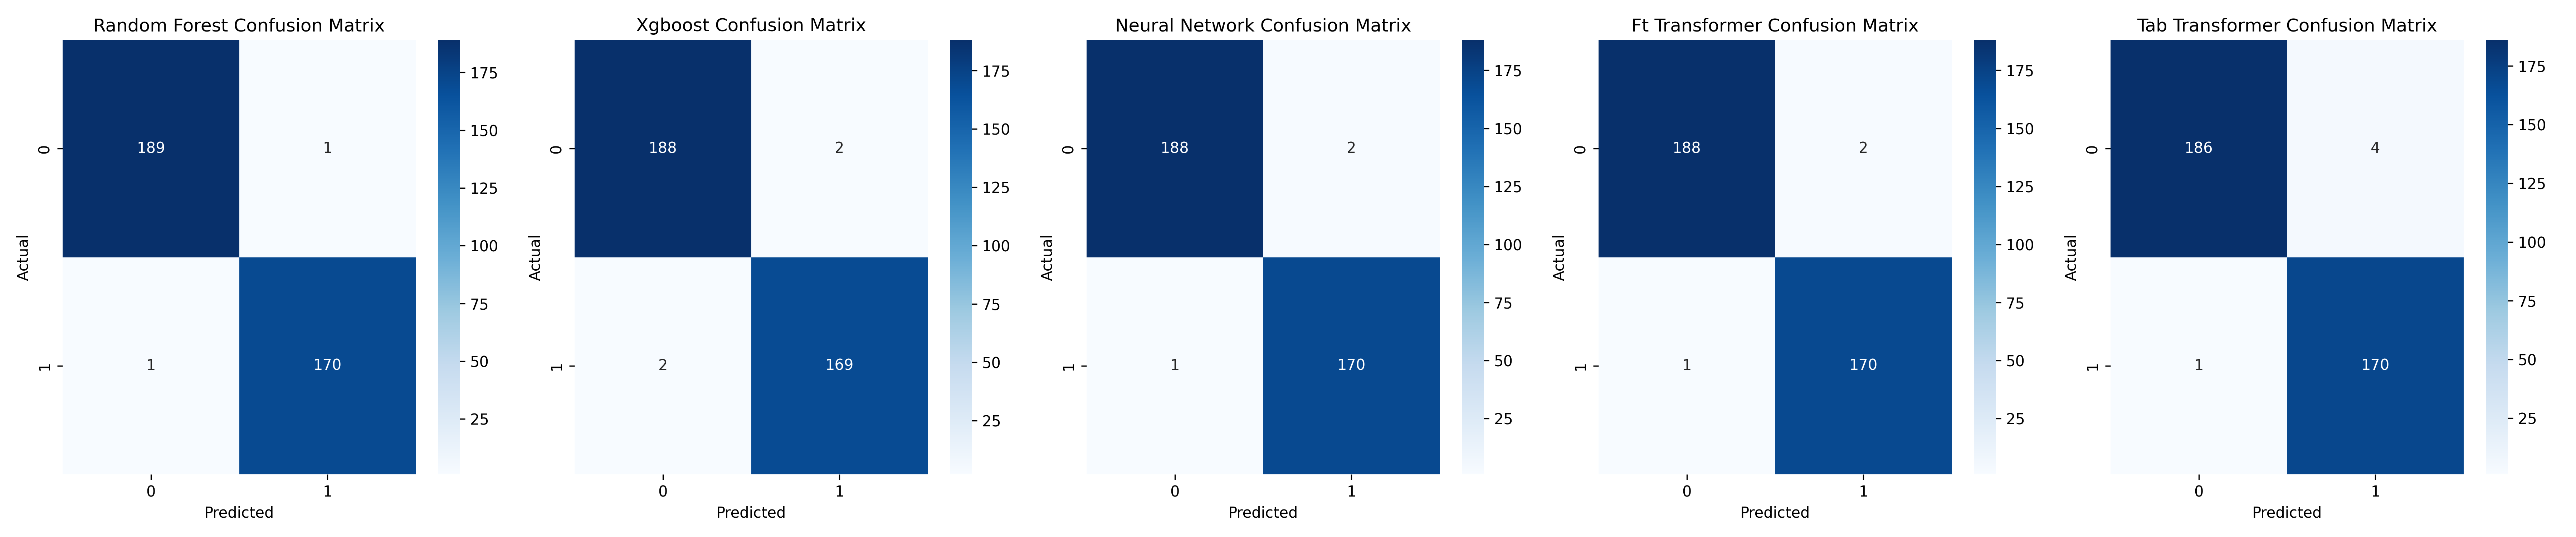
\includegraphics[width=\textwidth]{../images/ml_confusion_matrices.png} % Replace with your first image path
        \caption{Confusion Matrices}
        \label{fig:confusion_matrices_ml}
    \end{minipage}
    \hfill
    \begin{minipage}{0.45\textwidth}
        \centering
        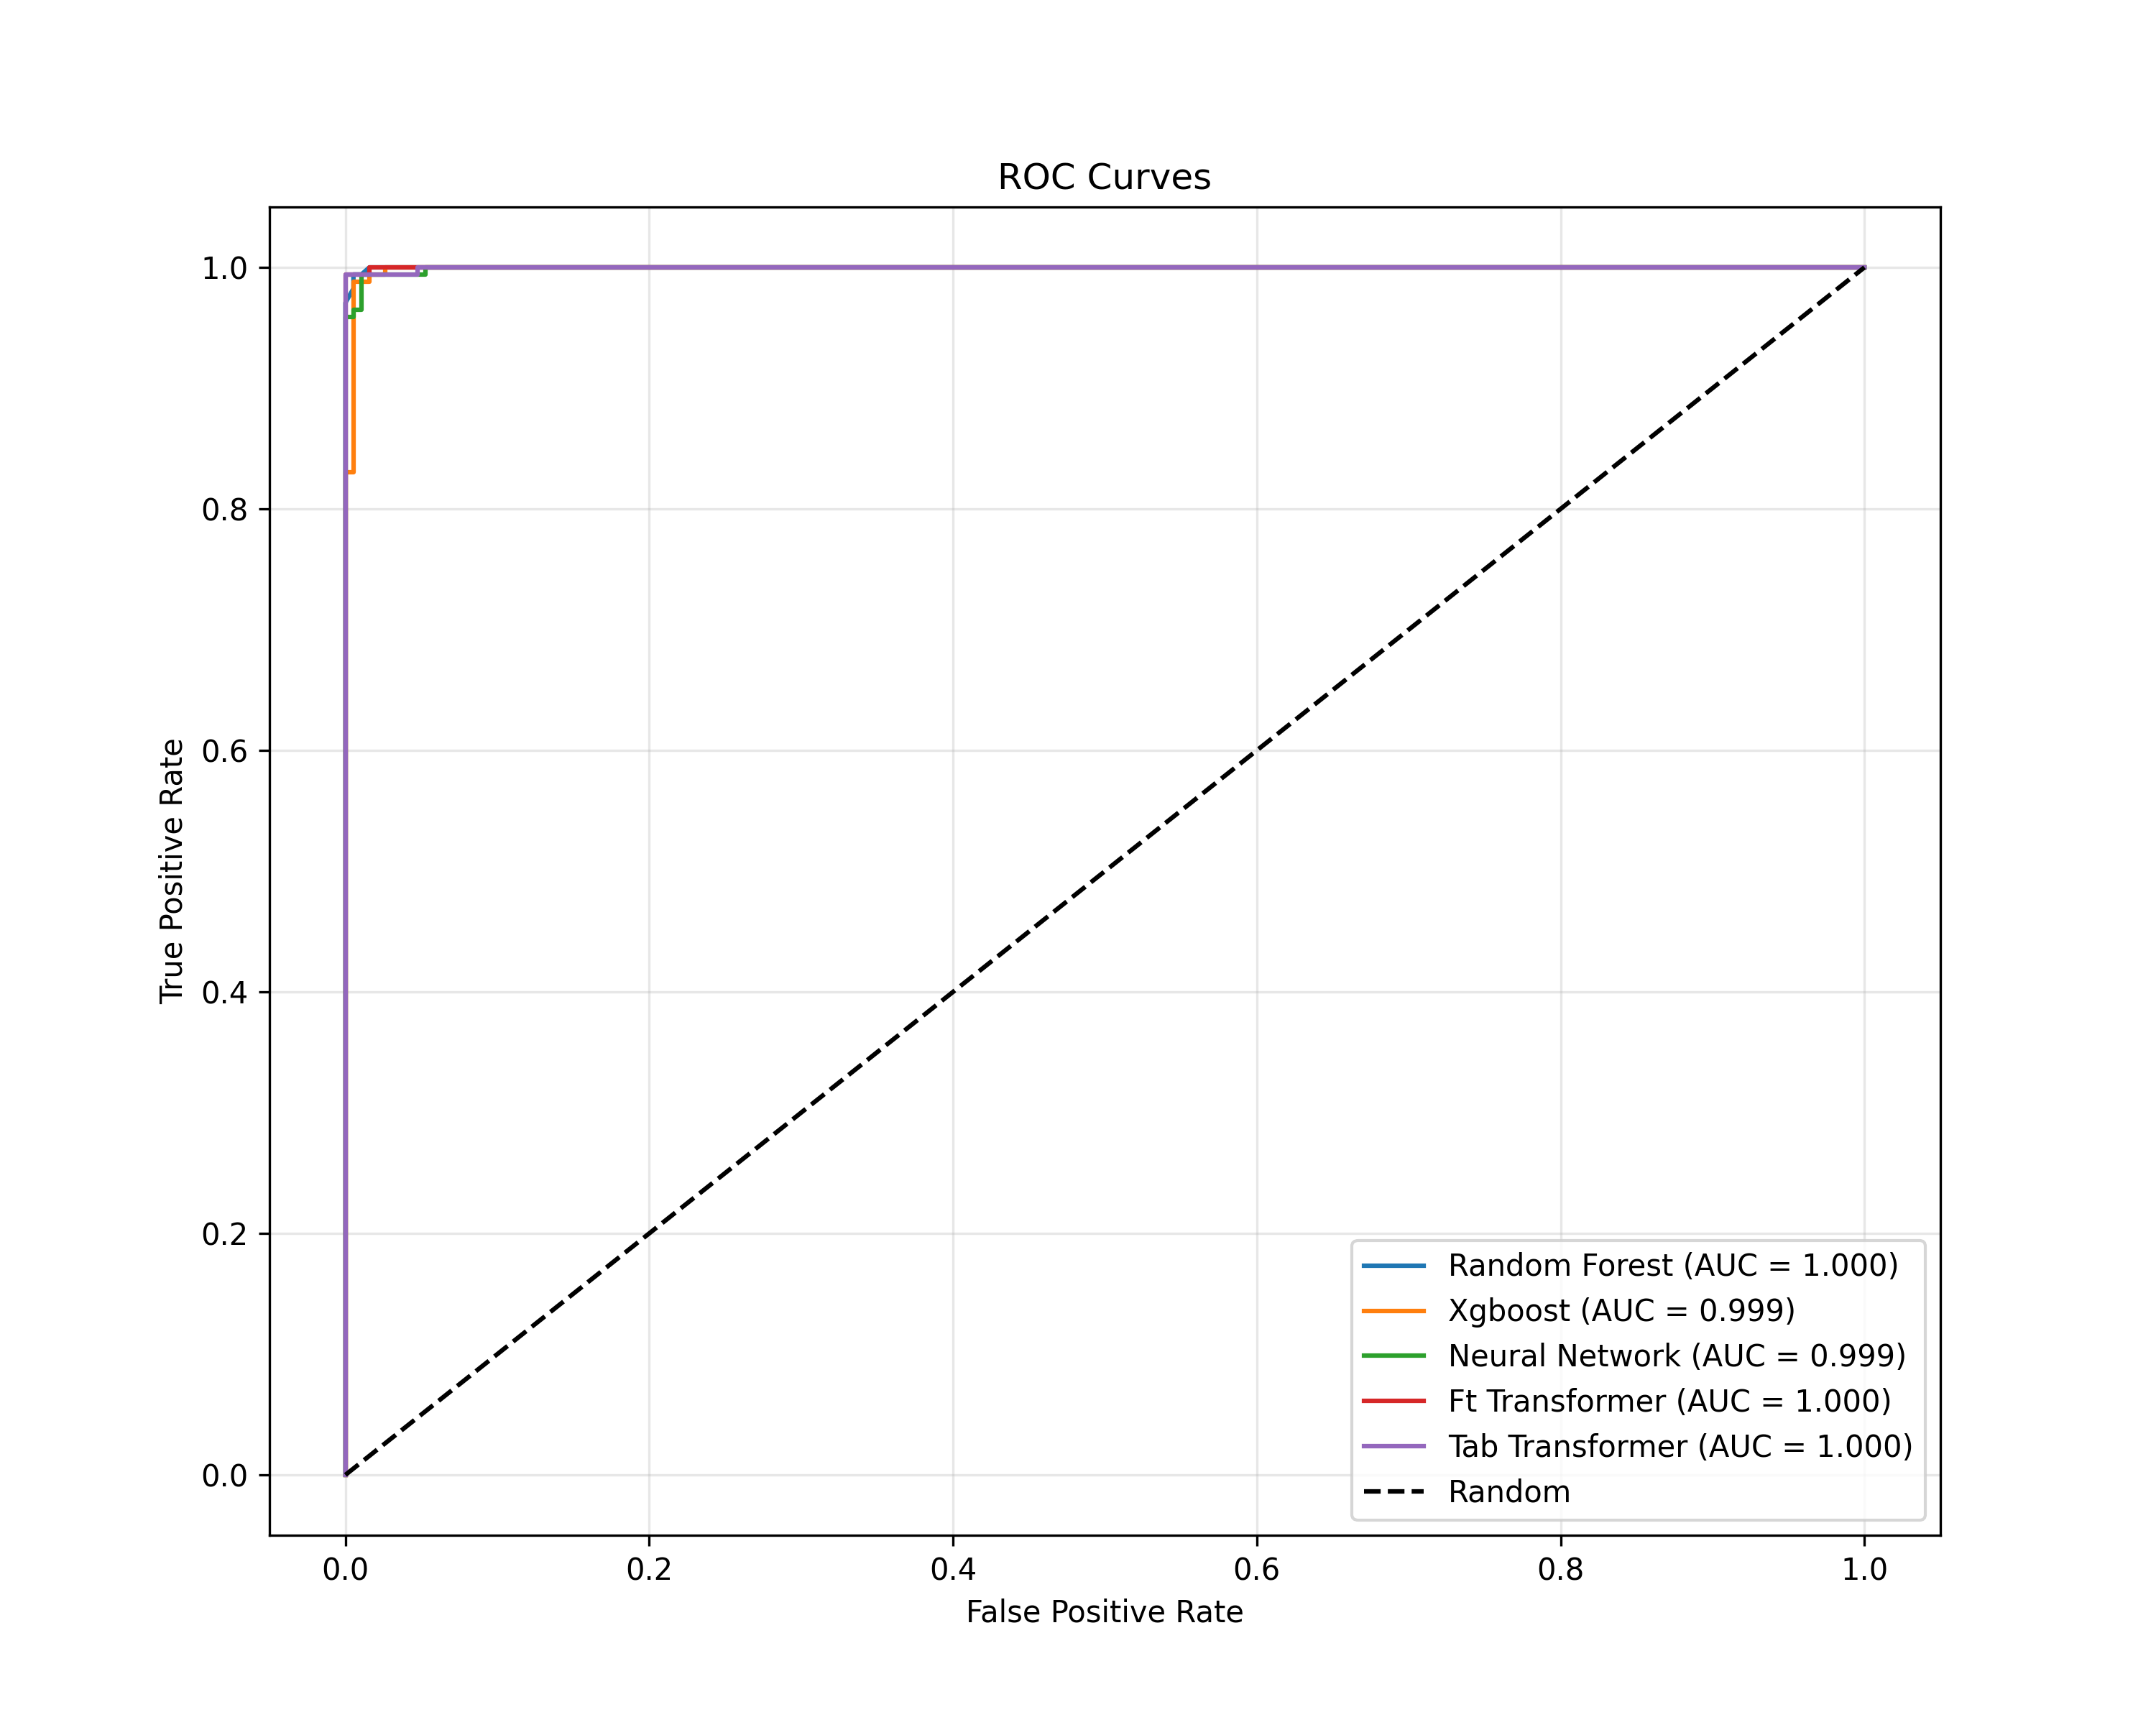
\includegraphics[width=\textwidth]{../images/ml_roc_curves.png} % Replace with your second image path
        \caption{ROC Curves}
        \label{fig:roc_curves_ml}
    \end{minipage}
\end{figure}

\subsection{AI-Assisted Interpretation of Deterioration Classification Results}

To augment the analysis, an AI model (\textit{Gemini-2.5-Flash-Thinking-Preview-0417}) \parencite{Doshi_2025} was employed to interpret the performance metrics table. The AI identified Random Forest as the best overall performer, attributing this to its superior accuracy, precision, recall, and F1-score, alongside a highly competitive AUC. While FT Transformer exhibited a marginally higher AUC, the AI emphasized Random Forest's balanced and consistently high scores across various threshold-dependent metrics. Comparing traditional and deep learning approaches, the AI noted that traditional tree-based models, particularly Random Forest and XGBoost, were highly competitive, with Random Forest leading. Among the deep learning models, FT Transformer achieved the best AUC, whereas Tab Transformer registered the lowest accuracy, precision, and F1-score. The AI attributed these performance differences to factors such as model suitability for tabular data (where tree-based models often excel), the capacity to capture complex feature interactions, model robustness (often enhanced by ensemble methods), the effectiveness of hyperparameter tuning, and the influence of data size. For further improvement, the AI suggested avenues including more rigorous hyperparameter tuning, comprehensive cross-validation, advanced feature engineering, the exploration of ensembling or stacking techniques, and fine-tuning of classification thresholds. Based on its analysis, the AI recommended Random Forest for potential deployment, citing its leading performance, inherent robustness, computational efficiency, and comparatively better interpretability in this context relative to the deep learning alternatives.

The AI's interpretation of the confusion matrices, based on raw True Negative (TN), False Positive (FP), False Negative (FN), and True Positive (TP) values, involved a recalculation of accuracy, precision, recall, and F1-scores. This re-evaluation positioned both Random Forest and FT Transformer as top performers. Random Forest demonstrated excellence in precision and overall accuracy. Notably, FT Transformer achieved perfect recall, successfully identifying all positive cases while maintaining high accuracy and F1-score. Tab Transformer also showed perfect recall but at the cost of lower precision. In contrast, XGBoost generally performed the worst according to these raw confusion matrix-derived metrics. The AI concluded that the "best" model selection would depend on specific clinical priorities: FT Transformer would be favored if minimizing False Negatives is paramount, whereas Random Forest would be preferred for minimizing False Positives or achieving a balanced F1-score.

An AI-driven interpretation of the ROC curves revealed that Random Forest, FT Transformer, and Tab Transformer all achieved perfect AUC scores of 1.000. XGBoost and Neural Network also demonstrated exceptional performance with AUCs of 0.999. The AI highlighted that such high AUC values imply an excellent to perfect ability of the models to distinguish between positive and negative classes on the evaluated dataset. However, these near-perfect scores prompted caution from the AI, which raised concerns regarding potential data leakage, overfitting (particularly if evaluation sets were small or cross-validation was not rigorously applied), or the possibility of a trivially easy dataset. Given that perfect scores were observed across multiple diverse architectures, data leakage was identified as a strong possibility requiring thorough investigation. The AI's report concluded that while all models exhibited outstanding performance on the provided evaluation set, the perfect or near-perfect AUCs warrant careful examination of potential underlying data issues before definitive conclusions about model robustness and generalizability can be drawn.

\subsection{Comparative Analysis and Discussion}

The models developed for patient deterioration classification generally demonstrated exceptionally high performance. As highlighted by both the initial results table and the AI's interpretation, the Random Forest model exhibited the most consistent and superior performance across accuracy, precision, recall, and F1-score. The FT Transformer also emerged as a strong contender, particularly distinguished by its leading AUC value.

The AI's recalculation of metrics directly from raw confusion matrix values offered a slightly more nuanced perspective, elevating FT Transformer to a similar top-tier status as Random Forest, with specific commendation for FT Transformer's perfect recall. This underscores that the interpretation of "best" performance can subtly shift depending on whether raw confusion matrix counts, pre-calculated metrics, or specific evaluation priorities (e.g., threshold-independent AUC versus threshold-dependent F1-score) are emphasized.

The achievement of perfect AUCs by three models—Random Forest, FT Transformer, and Tab Transformer—is particularly striking. As the AI interpretation correctly pointed out, such perfect scores, especially in a biomedical context even with simulated data, necessitate a meticulous review of the data generation, feature engineering, and data splitting processes. This review is crucial to rule out any form of data leakage or the creation of an overly simplistic classification task that might not accurately reflect real-world complexities. If these high scores are indeed genuine and the task is inherently highly separable with the given features, it would indicate that these models are exceptionally effective. Nevertheless, caution is advised. Further validation on more challenging, diverse, or independently generated datasets would be highly beneficial to confirm these findings. It is plausible that the engineered features derived from questionnaires and medical history significantly contributed to this high degree of separability observed in the data.

\subsection{NLP Task Results}

This sub-section details the performance of models developed for various NLP tasks, including sentiment analysis, clinical text interpretation (Named Entity Recognition), and questionnaire response classification, again incorporating AI-assisted interpretations.

\subsection{Sentiment Analysis on \texttt{describe\_lifestyle}}

For sentiment analysis, models were applied to the \texttt{describe\_lifestyle} text from questionnaire responses. Evaluation results which encompassed metrics for Fatigue, Activity/Anxiety, and Mental Health sentiment. The underlying models were BERT base, fine-tuned for 3-class sentiment classification (positive, neutral, negative). Visualizations included confusion matrices and ROC curves as well as training loss curves. The summary of evaluation metrics is presented in Table \ref{tab:sentiment_analysis_performance} below:

\begin{table}[htbp]
    \centering
    \caption{Performance Metrics of Sentiment Analysis Models}
    \label{tab:sentiment_analysis_performance}
    \begin{tabular}{lccccc}
        \hline
        \textbf{Model} & \textbf{Accuracy} & \textbf{Precision} & \textbf{Recall} & \textbf{F1-Score} & \textbf{AUC} \\
        \hline
        Fatigue & 0.917 & 0.922 & 0.917 & 0.918 & 0.923 \\
        Activity & 0.884 & 0.881 & 0.884 & 0.882 & 0.887 \\
        Mental Health & 0.888 & 0.890 & 0.888 & 0.889 & 0.890 \\
        \hline
    \end{tabular}
\end{table}

AI-assisted interpretations provided further insights. The AI rated the AUC, Figure \ref{fig:confusion_matrices_sa} for Fatigue (0.92) as excellent, and those for Activity/Anxiety (0.89) and Mental Health (0.89) as very good, indicating strong discriminatory power for all models. Fatigue's superior performance was hypothesized to stem from potentially clearer linguistic patterns or less ambiguity within its associated dataset. Analysis of confusion matrices, Figure \ref{fig:roc_curves_sa} revealed that the Fatigue model performed excellently on True Positives and True Negatives, with its main weakness being the Neutral class. The Activity/Anxiety model was strong on True Negatives but struggled significantly with the Neutral class and exhibited more diffuse errors. The Mental Health model showed outstanding performance on True Positives, with its primary weakness also being the Neutral class. The AI also flagged "Activity" as a likely typo for "Anxiety." Class imbalance and sentiment overlap, especially concerning the "Neutral" category, were identified as potential contributing issues. Interpretation of the loss curves indicated that all models learned effectively from the training data. However, severe overfitting was observed early in training (around Epoch 2-3), Figure \ref{fig:loss_curves_sa} for all categories, evidenced by validation loss increasing or fluctuating while training loss continued to decrease. This suggested that training for the full 30 epochs was excessive, and early stopping at the best epoch (Epoch 2 or 3, depending on the category) was deemed crucial. The AI recommended strategies such as early stopping, regularization, acquiring more data, and adjusting learning rates to mitigate overfitting. The AI's interpretation of aggregated metrics confirmed the Fatigue model as the strongest performer across all metrics, with Mental Health slightly outperforming Activity. While these aggregate metrics aligned with ROC and confusion matrix findings, they tended to mask per-class struggles, particularly with the 'Moderate Risk' (likely corresponding to 'Neutral' sentiment) class. Limitations due to the small dataset size and the inherent subjectivity of questionnaire data were also noted by the AI.

\begin{figure}[httpb] % 'b' places the figure at the bottom of the page
    \centering
    \begin{minipage}{0.45\textwidth}
        \centering
        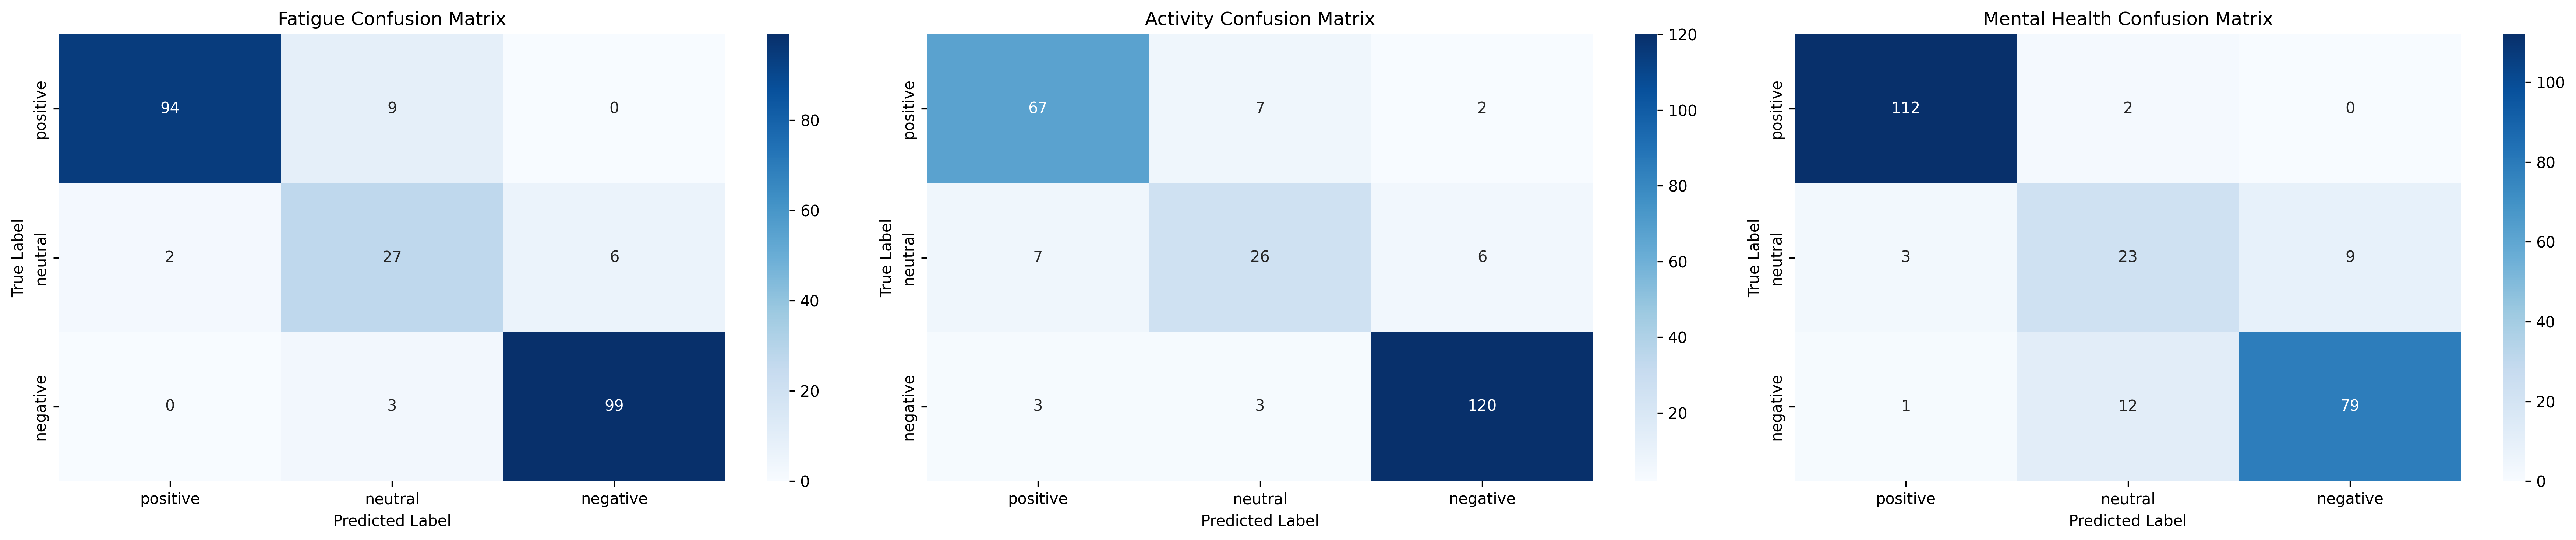
\includegraphics[width=\textwidth]{../images/sa_confusion_matrices.png} % Replace with your first image path
        \caption{Confusion Matrices}
        \label{fig:confusion_matrices_sa}
    \end{minipage}
    \hfill
    \begin{minipage}{0.45\textwidth}
        \centering
        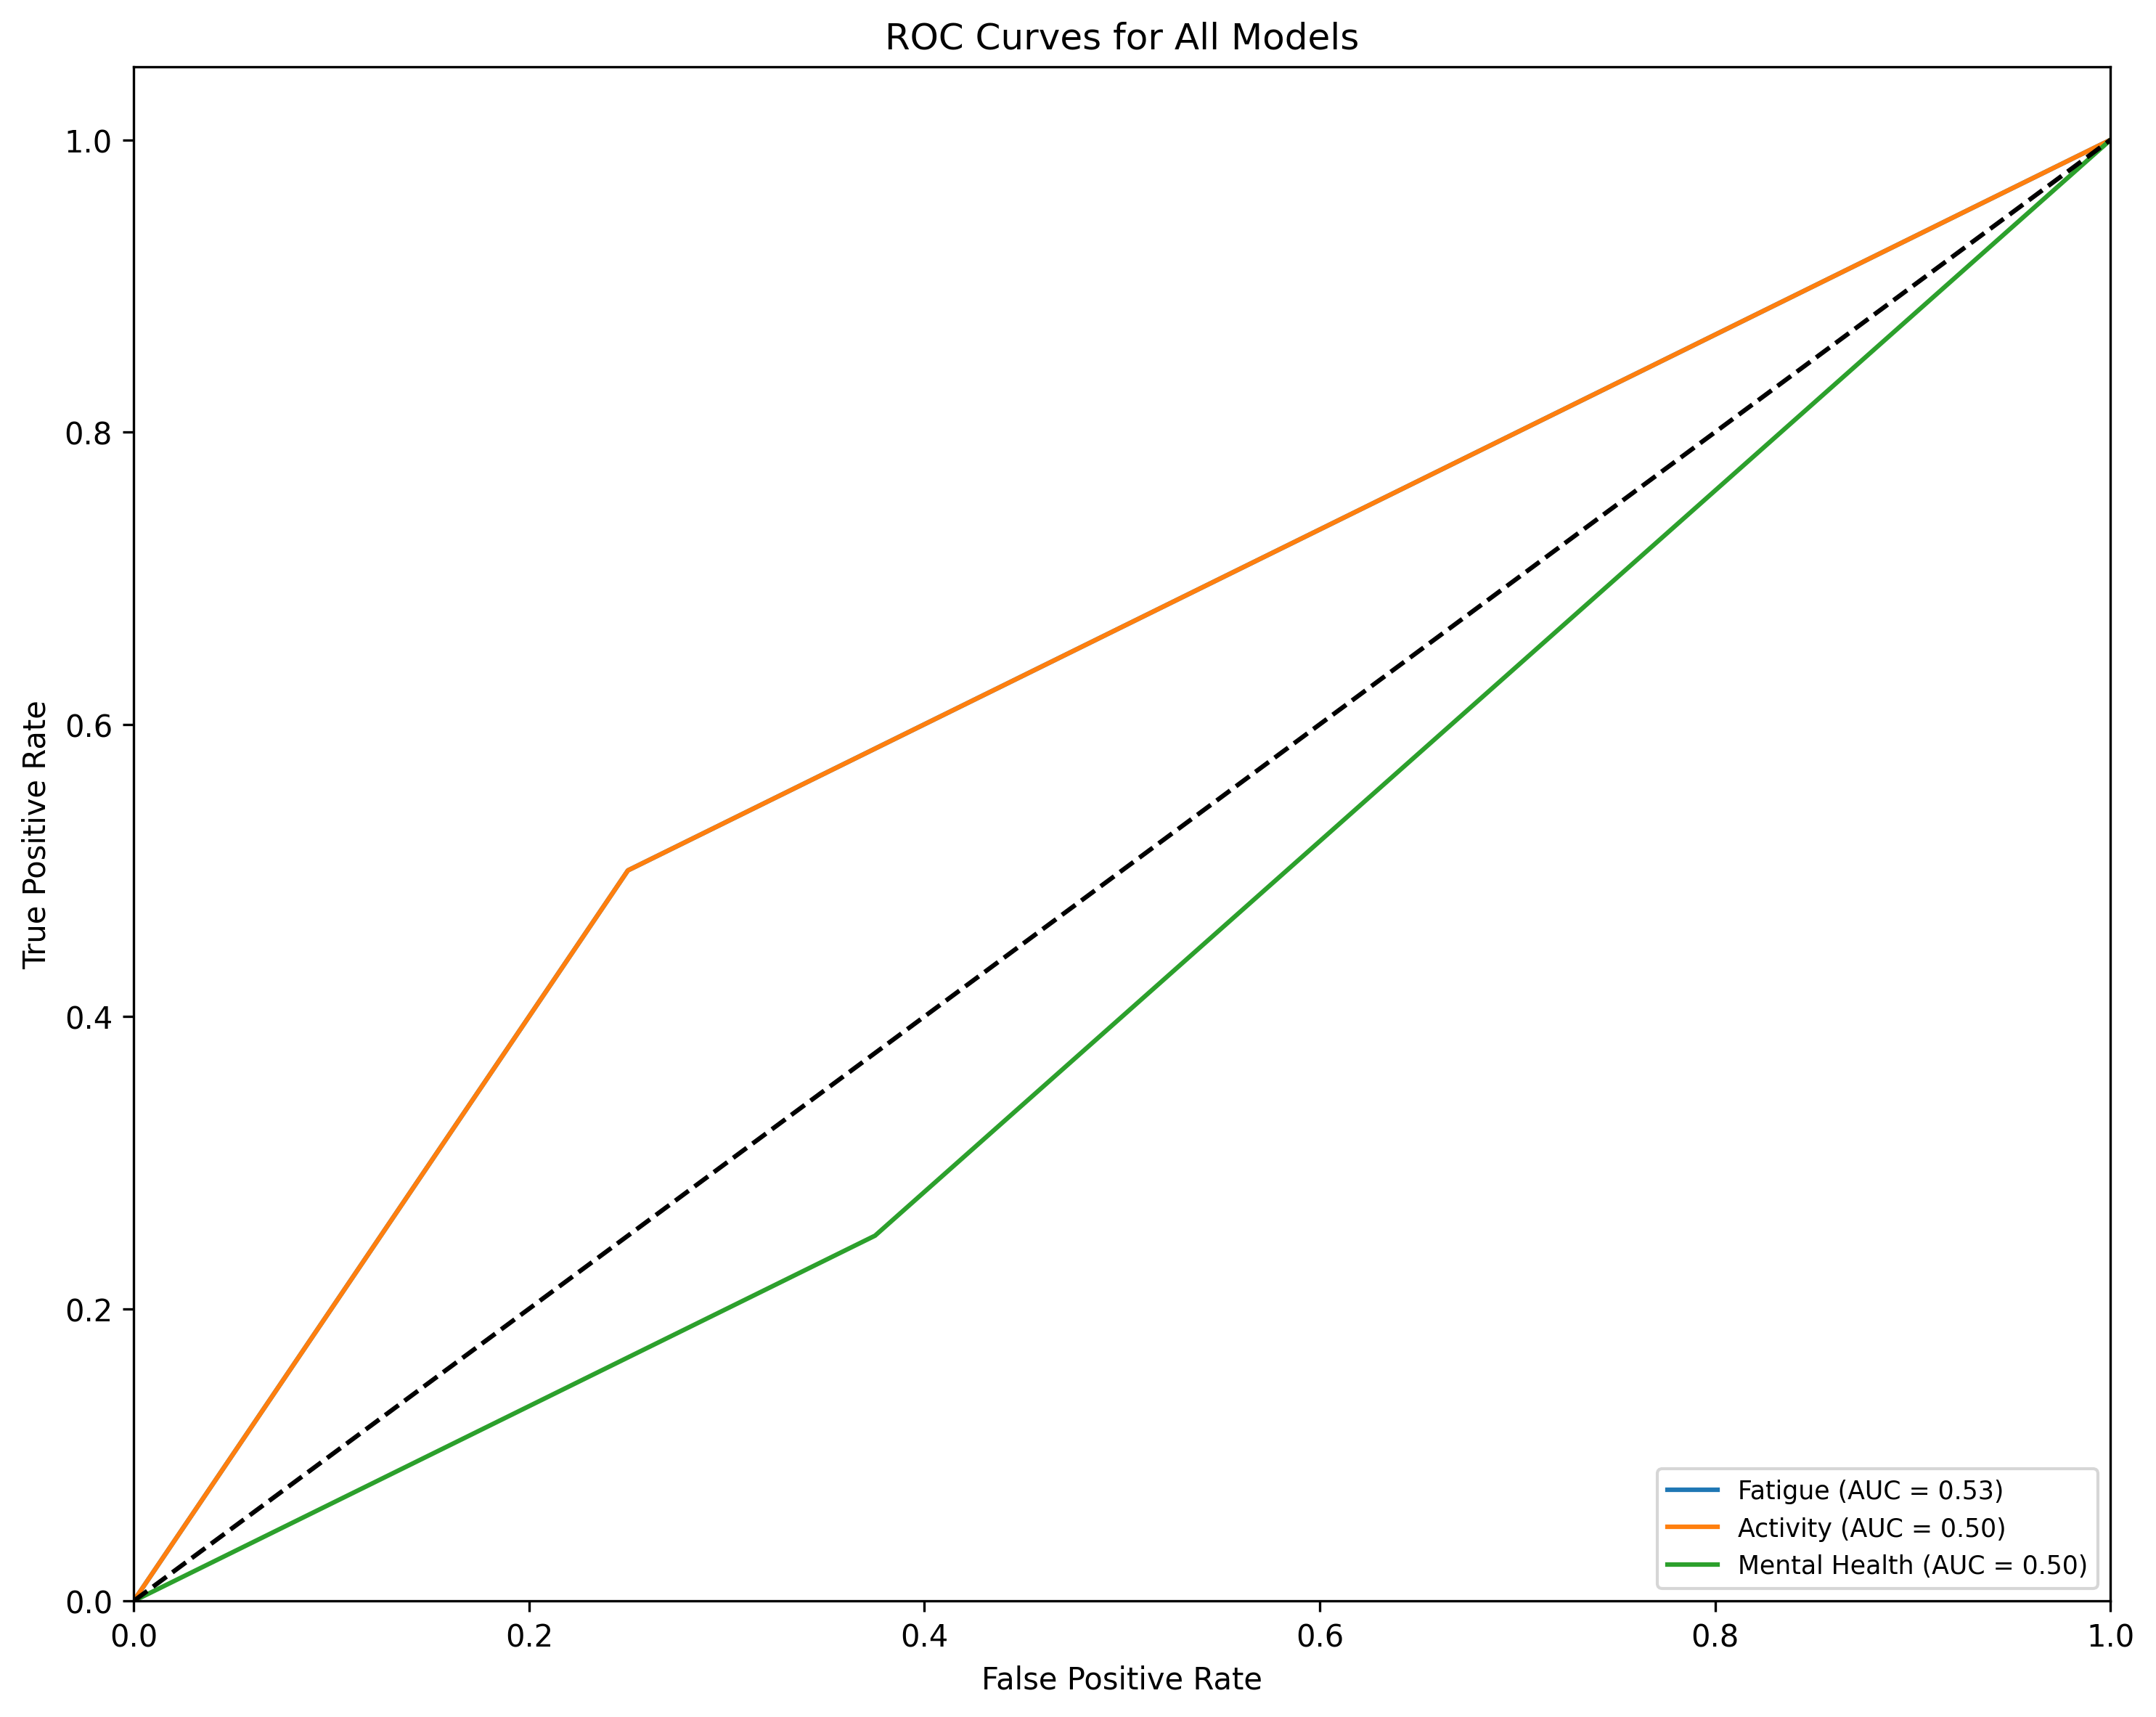
\includegraphics[width=\textwidth]{../images/sa_roc_curves.png} % Replace with your second image path
        \caption{ROC Curves}
        \label{fig:roc_curves_sa}
    \end{minipage}
\end{figure}

\begin{figure}[htpb]
    \centering
    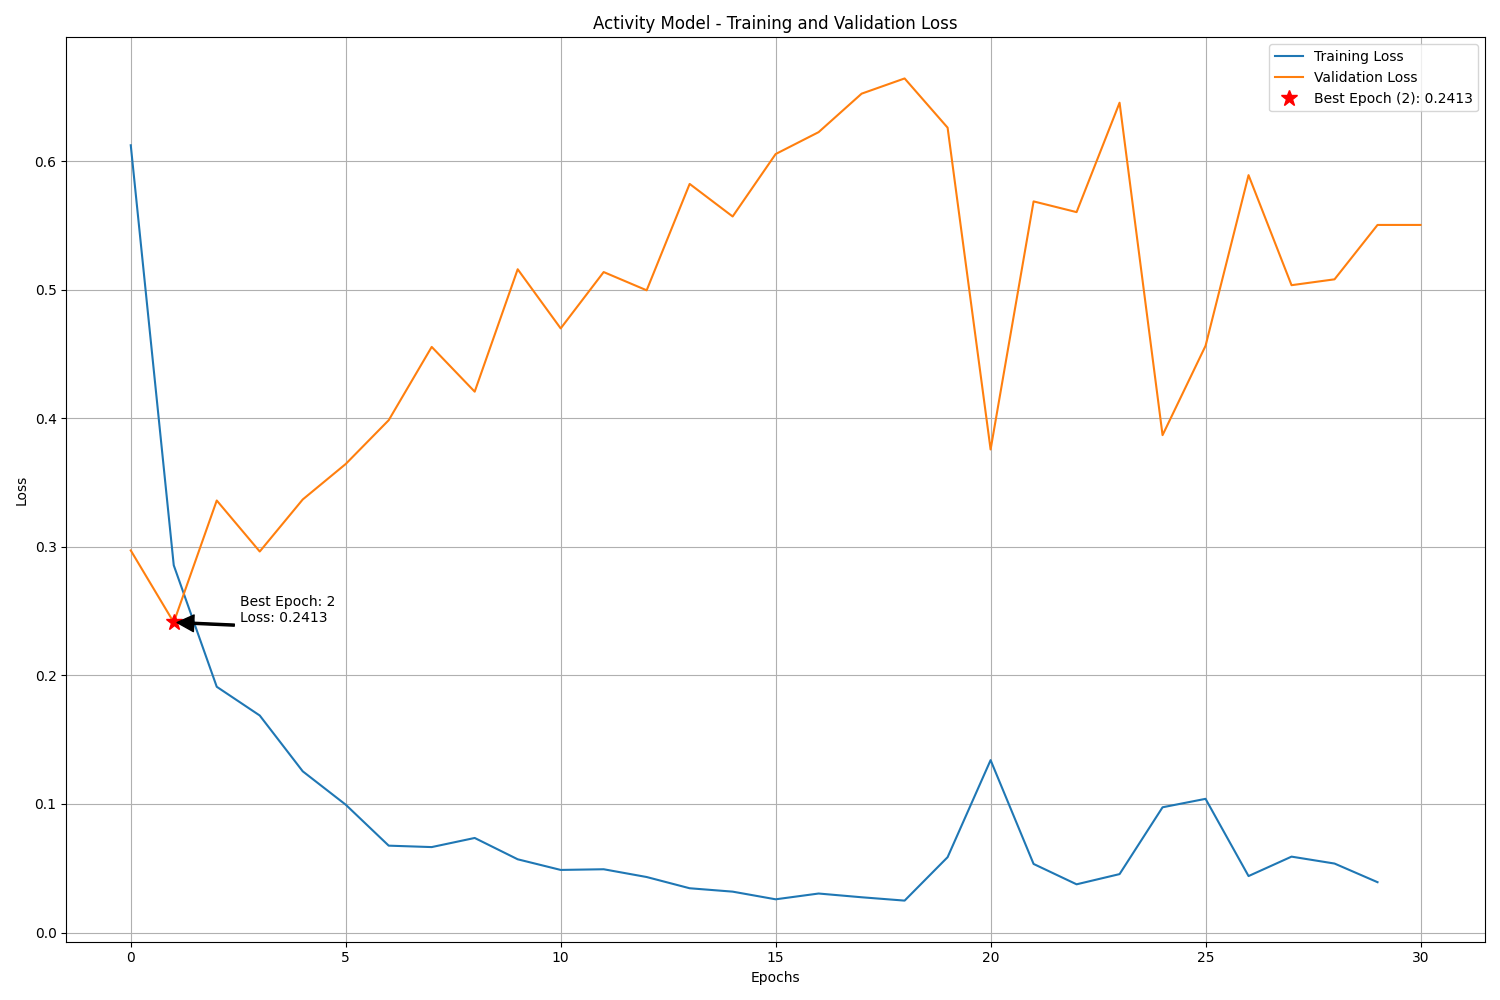
\includegraphics[width=0.4\textwidth]{../images/sa_loss_curves_with_best_epoch.png} % Replace with your image path
    \caption{Training Loss Curves with Best Epoch}
    \label{fig:loss_curves_sa}
\end{figure}

In discussion, the BERT base models demonstrated commendable performance in sentiment analysis, particularly for the Fatigue category. A consistent challenge across all sentiment categories was the classification of "Neutral" sentiment, a common difficulty in NLP tasks due to its subjective nature and often subtle linguistic expression. The early and pronounced overfitting highlighted by the AI's analysis of loss curves suggests that even robust models like BERT base can quickly memorize training examples when datasets are small, underscoring the critical importance of careful early stopping procedures.

\subsection{Clinical Text Interpretation (NER) on medical\_history}

Named Entity Recognition (NER) was performed on medical\_history text using a fine-tuned Bio-Clinical BERT model. The notebook loaded NER evaluation results in cell 497826f3, summarized in the Metrics Table \ref{tab:ner_performance} below:

\begin{table}[htbp]
    \centering
    \caption{Performance Metrics of Named Entity Recognition Model}
    \label{tab:ner_performance}
    \begin{tabular}{lccccc}
        \hline
        \textbf{Model} & \textbf{Accuracy} & \textbf{Precision} & \textbf{Recall} & \textbf{F1-Score} & \textbf{AUC} \\
        \hline
        Bio-Clinical BERT & 0.998 & 0.908 & 0.943 & 0.926 & 1.000 \\
        \hline
    \end{tabular}
\end{table}

The ROC curve, Figure \ref{fig:ner_roc_curve} for this task indicated an AUC of 1.00. Training curves, Figure \ref{fig:ner_training_curves}, provided insights into the learning process.

\begin{figure}[httpb] % 'b' places the figure at the bottom of the page
    \centering
    \begin{minipage}{0.45\textwidth}
        \centering
        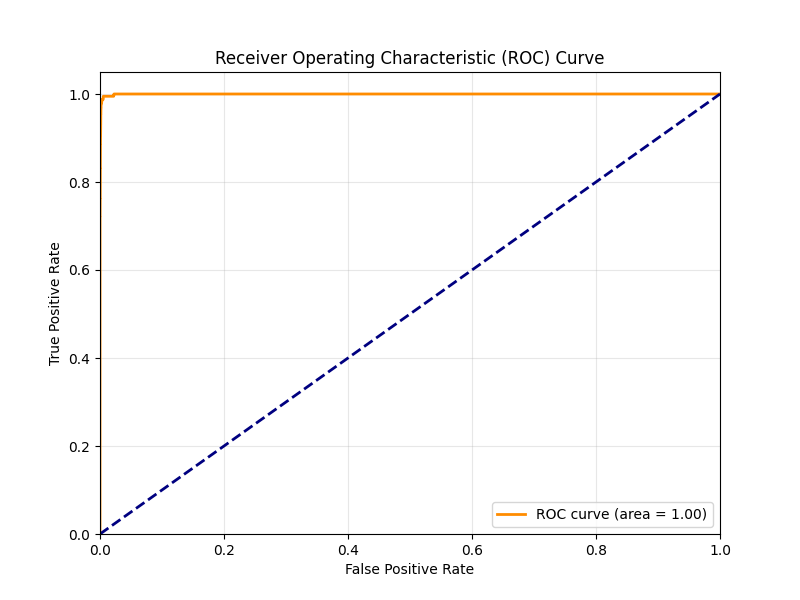
\includegraphics[width=\textwidth]{../images/ner_roc_curve.png} % Replace with your first image path
        \caption{ROC Curve}
        \label{fig:ner_roc_curve}
    \end{minipage}
    \hfill
    \begin{minipage}{0.45\textwidth}
        \centering
        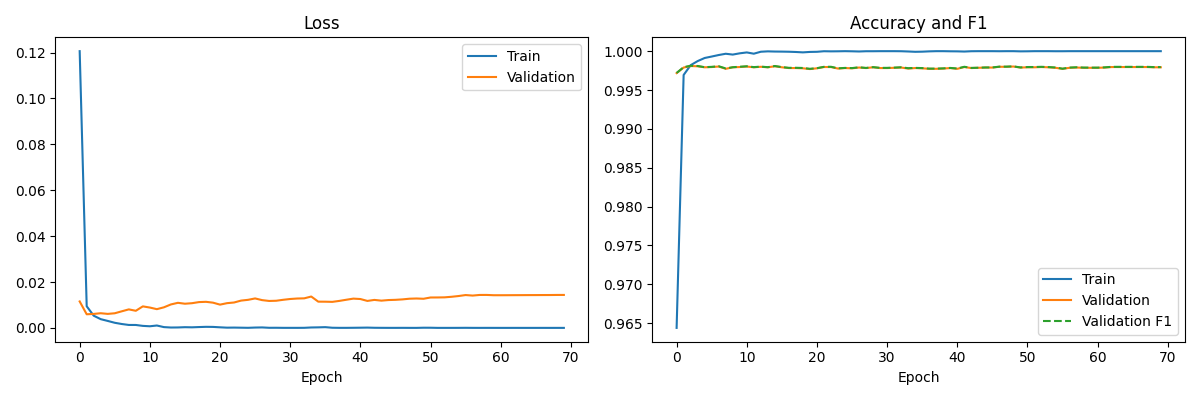
\includegraphics[width=\textwidth]{../images/ner_training_curves.png} % Replace with your second image path
        \caption{Training Curves}
        \label{fig:ner_training_curves}
    \end{minipage}
\end{figure}

AI-assisted interpretations offered a detailed analysis. The AI noted the exceptionally high accuracy (99.8\%), high F1-score (92.6\%), excellent recall (94.3\%), and good precision (90.8\%). The AUC (0.9996 from the Table \ref{tab:ner_performance}, 1.00 from the Figure \ref{fig:ner_roc_curve}) suggested near-perfect discriminative power at the token level for identifying entity tokens versus non-entity tokens. The AI cautioned that the high accuracy could be influenced by the preponderance of non-entity tokens (the "O" tag in IOB notation). High recall was deemed crucial for minimizing missed entities, while high precision indicated that most extracted entities were correct, with a slight observed preference for recall over precision. The AI's interpretation of the ROC curve, showing an AUC of 1.00 (or 0.9996), pointed to a perfect or near-perfect classifier at the token level. However, this perfect score again raised concerns about potential data leakage or an overly simplistic sub-problem, especially considering the high performance across other metrics. The AI's analysis of the training curves revealed that training loss dropped rapidly to near zero, and training accuracy/F1 reached near 1.0 very quickly, indicating that the model had effectively mastered the training data. Validation loss also decreased but plateaued at a level higher than training loss, signaling some degree of overfitting. Validation accuracy and F1-score were extremely high (approximately 0.998). A significant discrepancy was highlighted by the AI between the validation F1-score (0.998) observed from these training plots and the test F1-score (0.926) reported from the independent test set. This disparity strongly suggested poor generalization from the (small) training/validation data to the test set, likely attributable to the very small dataset size (1000 data points for NER). Consequently, the AI's recommendations heavily emphasized the need for acquiring more data, employing data augmentation techniques, and implementing robust cross-validation, given the dataset limitations.

Discussing these findings, the Bio-Clinical BERT model demonstrated very high potential for NER on disease entities. Token-level metrics such as Accuracy and the AUC derived from the ROC curve were near-perfect. However, the entity-level F1-score, while good at 0.926, was considerably lower than the F1-score observed on the validation set during training. This discrepancy highlights a common challenge when working with small datasets: a model can appear to perform almost perfectly on validation data but still struggle to generalize effectively to a truly independent test set, particularly for complex sequence labeling tasks like NER. The observed drop of approximately 7\% in F1-score indicates that while token-level classification might be excellent, consistently and correctly identifying the exact boundaries and types of entities on new, unseen data proves more challenging.

\subsection{Questionnaire Response Classification (\texttt{describe\_fatigue\_level, describe\_mental\_health})}

This task involved using BERT base models to classify textual questionnaire responses from \texttt{describe\_fatigue\_level} and \texttt{describe\_mental\_health} into "Low Risk," "Moderate Risk," and "High Risk" categories. The results and discussion for this appear to align closely with those presented for the "Sentiment Analysis" task, where "Fatigue," "Activity/Anxiety," and "Mental Health" were the evaluated categories with labels "positive," "neutral," and "negative." It is assumed that a mapping exists, such as "positive" to "Low Risk," "neutral" to "Moderate Risk," and "negative" to "High Risk," or a similar schema appropriate to the problem's framing. Therefore, the discussion from sentiment analysis largely applies here. Visual performance indicators for this specific framing are provided by confusion matrices, Figure \ref{fig:qr_confusion_matrices} and ROC curves, Figure \ref{fig:qr_roc_curves}.

\begin{figure}[httpb] % 'b' places the figure at the bottom of the page
    \centering
    \begin{minipage}{0.45\textwidth}
        \centering
        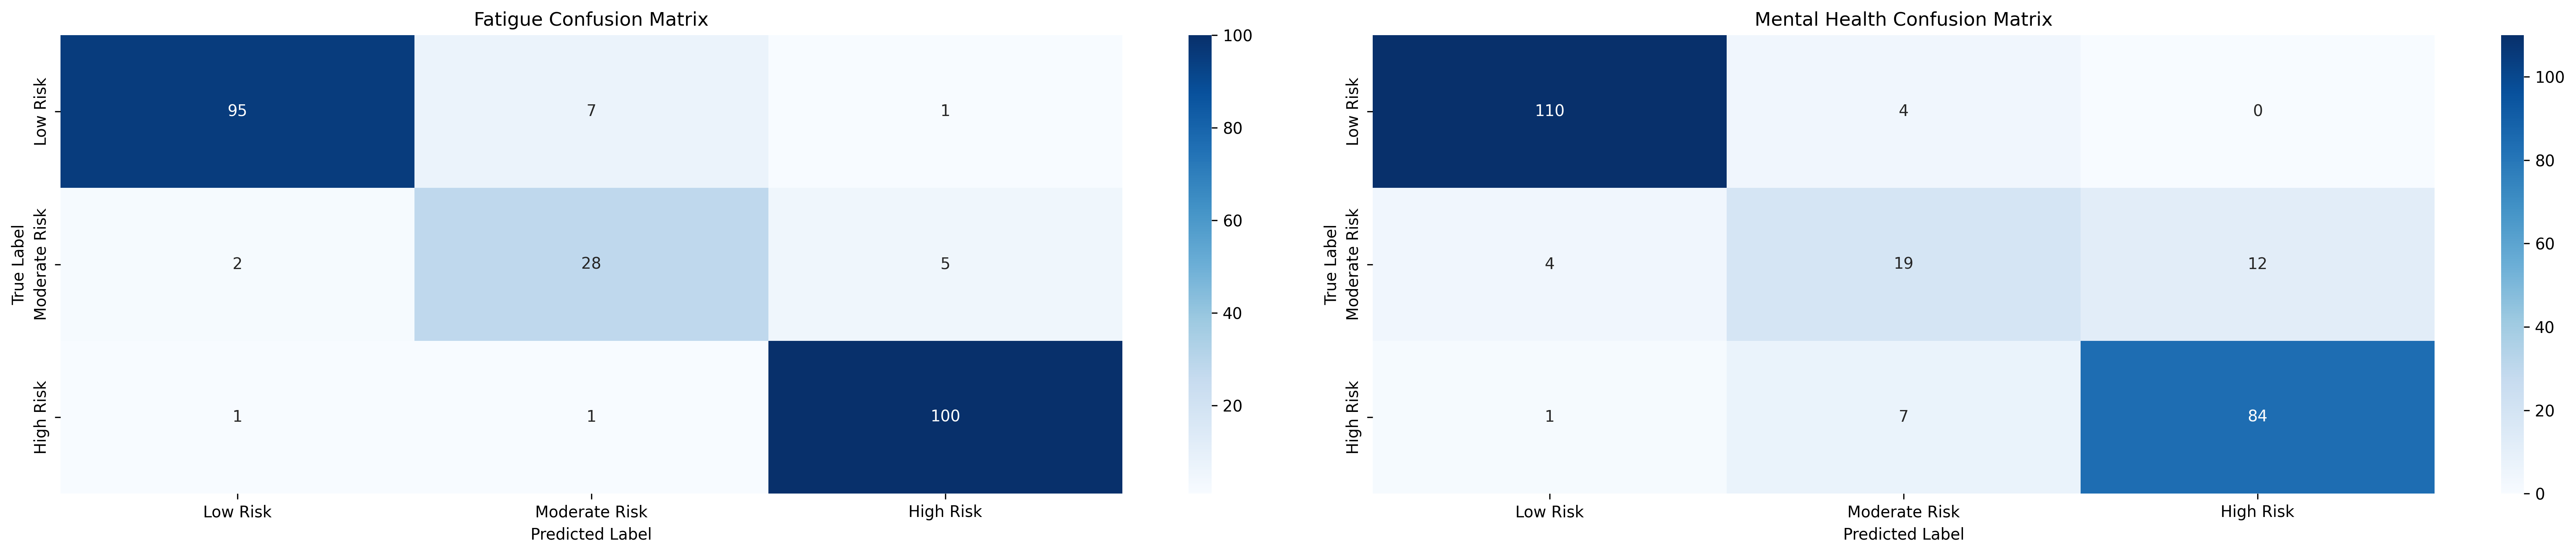
\includegraphics[width=\textwidth]{../images/qr_confusion_matrices.png} % Replace with your first image path
        \caption{Confusion Matrices}
        \label{fig:qr_confusion_matrices}
    \end{minipage}
    \hfill
    \begin{minipage}{0.45\textwidth}
        \centering
        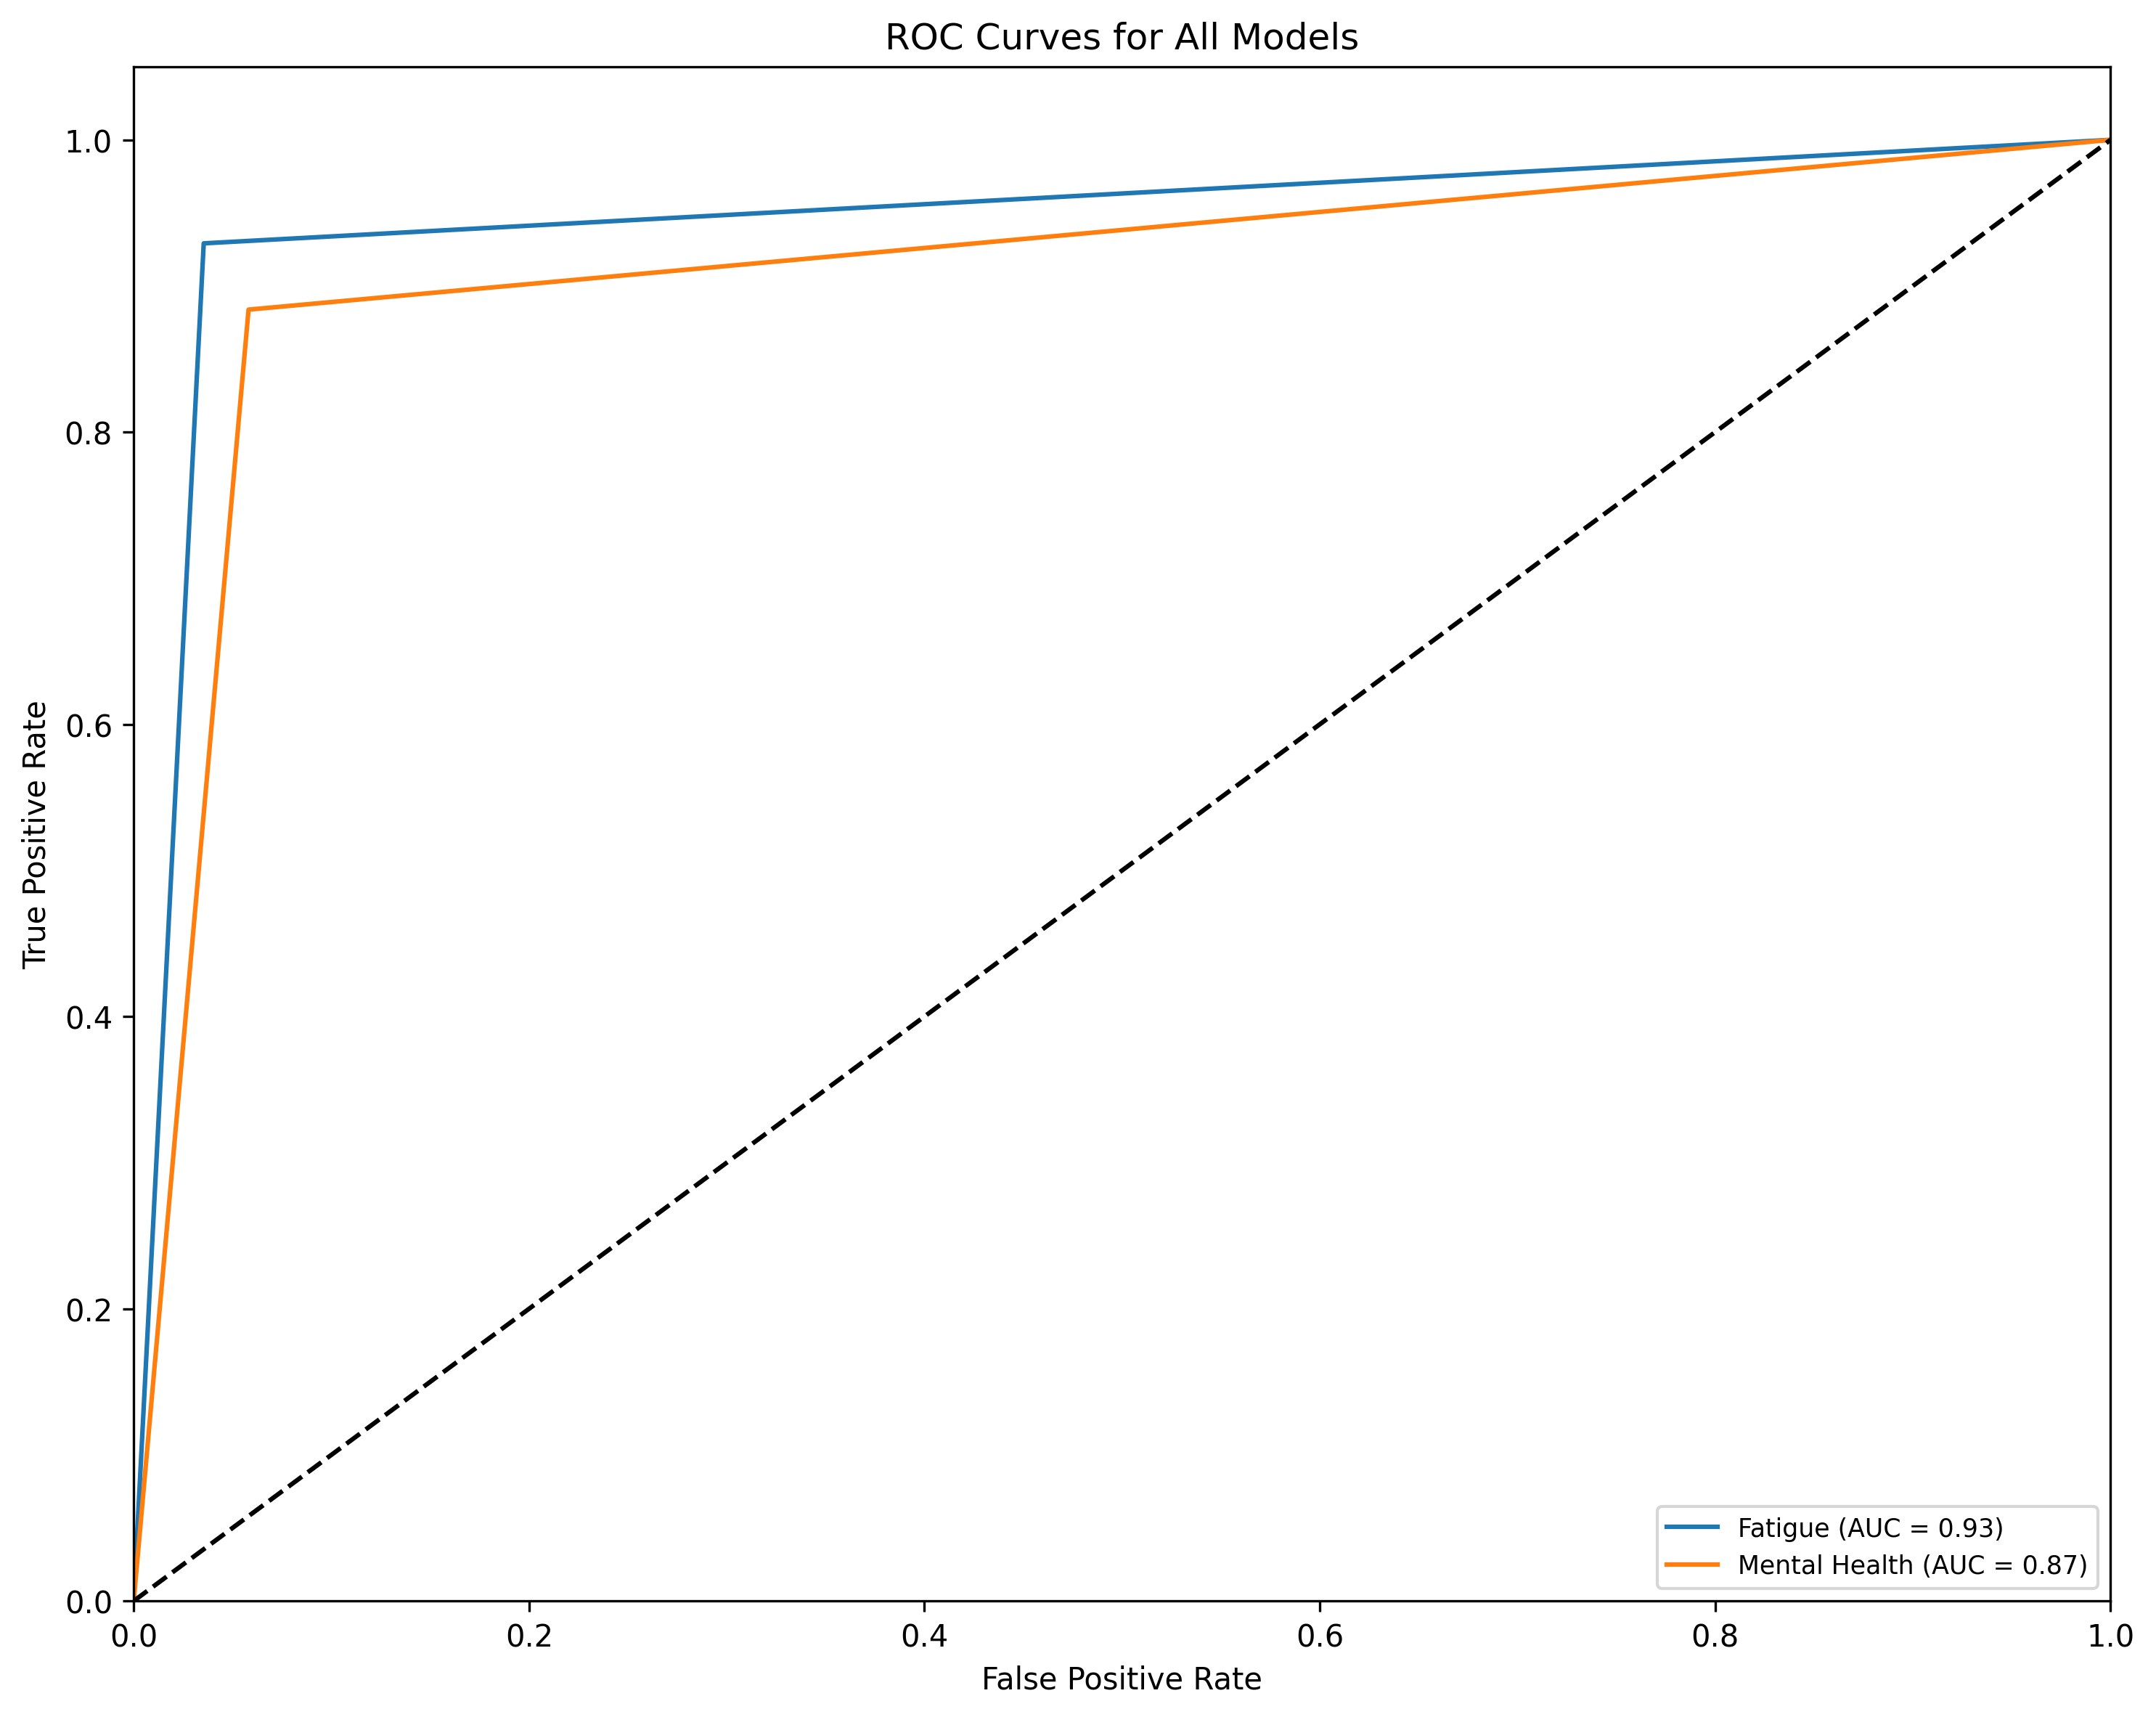
\includegraphics[width=\textwidth]{../images/qr_roc_curves.png} % Replace with your second image path
        \caption{ROC Curves}
        \label{fig:qr_roc_curves}
    \end{minipage}
\end{figure}

AI-assisted interpretation provided specific insights for this risk classification task. The AI calculated accuracies of approximately 92.9\% for Fatigue and 88.4\% for Mental Health from the confusion matrices. Both models demonstrated strength in identifying 'High Risk' cases (high recall). However, the 'Moderate Risk' class emerged as the weakest link for both models, suffering from numerous misclassifications into either 'Low' or 'High' risk categories. A critical error was noted for the Mental Health model, which misclassified 2 True High Risk cases as Low Risk. Class imbalance, with the 'Moderate Risk' category being smaller, was identified by the AI as a key contributing issue. Interpretation of the ROC curves indicated an AUC of 0.93 (excellent) for Fatigue and 0.87 (very good) for Mental Health, with the Fatigue model showing superior overall discriminative power. The AI also discussed limitations related to the small dataset size and the inherent nature of multi-class ROC calculation (e.g., reliance on One-vs-Rest averaging). The model evaluation metrics is shown in Table \ref{tab:questionnaire_risk_performance} below:

\begin{table}[htbp]
    \centering
    \caption{Performance Metrics of Questionnaire Risk Classification Models}
    \label{tab:questionnaire_risk_performance}
    \begin{tabular}{lccccc}
        \hline
        \textbf{Model} & \textbf{Accuracy} & \textbf{Precision} & \textbf{Recall} & \textbf{F1-Score} & \textbf{AUC} \\
        \hline
        Fatigue & 0.929 & 0.932 & 0.929 & 0.930 & 0.933 \\
        Mental Health & 0.884 & 0.877 & 0.884 & 0.878 & 0.871 \\
        \hline
    \end{tabular}
\end{table}

In summary, the BERT models were effective in stratifying risk levels based on textual questionnaire responses, particularly for the Fatigue category. The 'Moderate Risk' category consistently proved challenging, a common phenomenon in multi-class classification problems involving ordinal or subjective labels, often exacerbated by class imbalance. The observed performance disparity, Figure \ref{fig:qr_loss_curves} between the Fatigue and Mental Health models suggests that the linguistic cues indicative of fatigue risk might be more distinct or easier for the model to learn from the limited available data compared to those signaling mental health risk.

\begin{figure}[htpb]
    \centering
    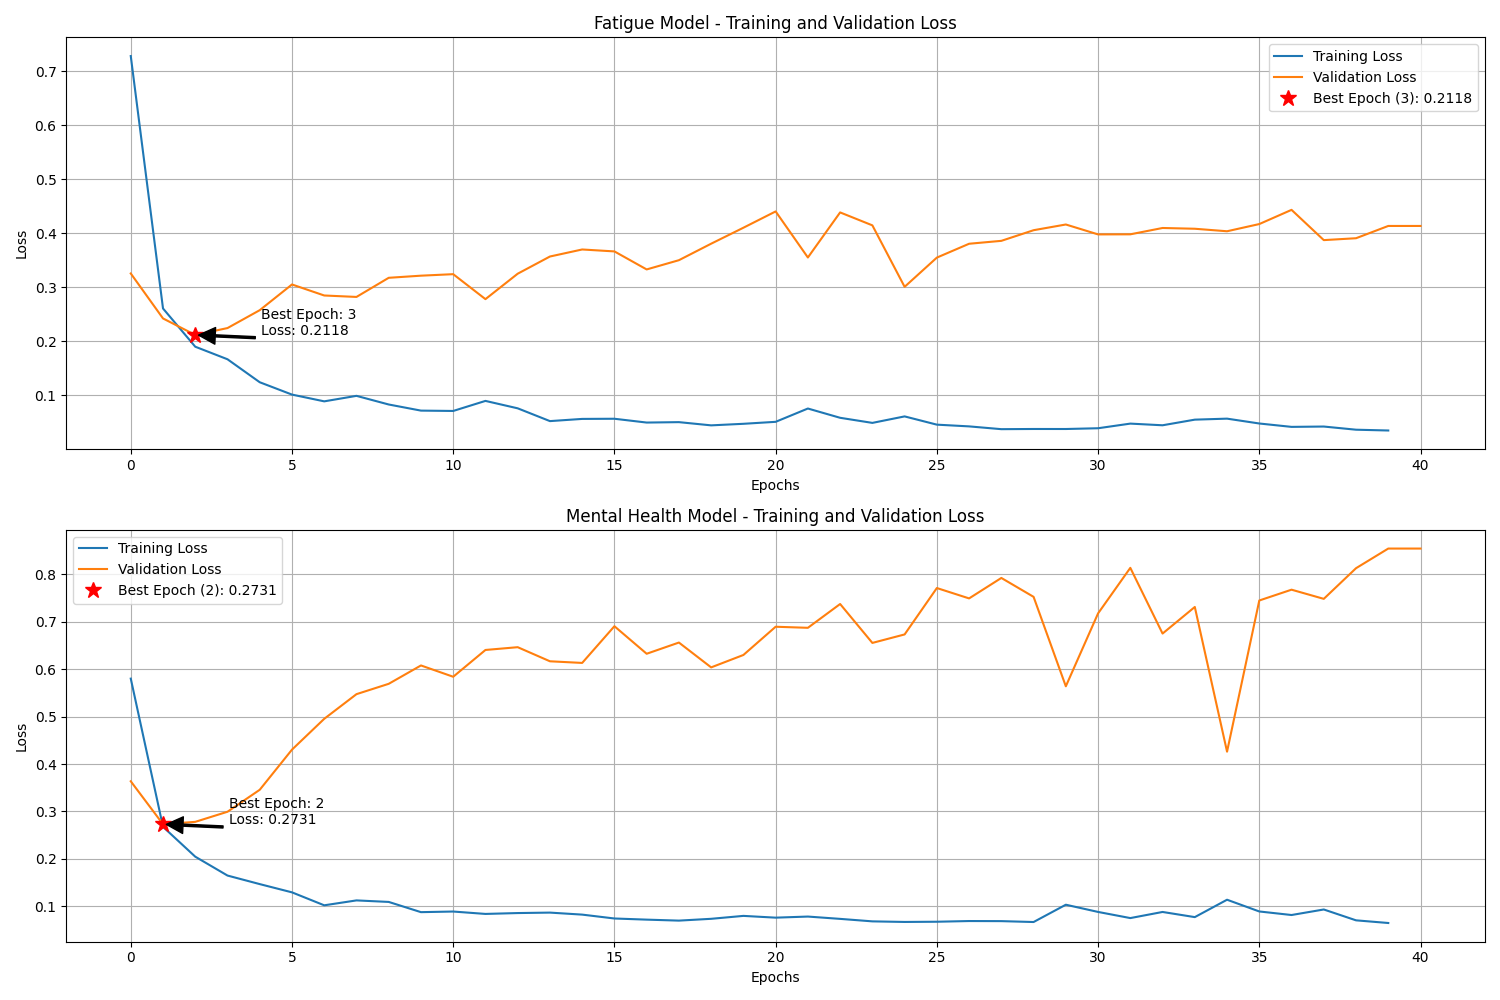
\includegraphics[width=0.4\textwidth]{../images/qr_loss_curves_with_best_epoch.png} % Replace with your image path
    \caption{Training Loss Curves with Best Epoch}
    \label{fig:qr_loss_curves}
\end{figure}

\subsection{Overall Discussion}

This section synthesizes the findings from both patient deterioration classification and the various NLP tasks, discussing their contributions, the role of generative AI and large language models, and persistent challenges.

The project successfully demonstrated the application of diverse AI models for the prediction of patient deterioration and a suite of related NLP tasks. Transformer-based models, notably FT Transformer for tabular data and various BERT variants for NLP applications, exhibited strong performance across their respective domains. The NLP tasks were crucial in generating quantifiable features, such as recognized disease entities from medical history (NER) and severity scores derived from questionnaire responses, as well as providing direct risk or sentiment classifications from free-text inputs.

While the contribution of NLP-derived features to the patient deterioration prediction models was not explicitly quantified through ablation studies in the provided notebook, their integral role is evident. Features engineered from \texttt{medical\_history} (e.g., extracted diseases via NER) and \texttt{questionnaire\_responses} (e.g., sentiment or risk severity scores) served as key inputs to the deterioration models. The exceptionally high performance of these models, exemplified by AUCs consistently exceeding 0.99, strongly suggests that these NLP-derived features were highly informative and contributed significantly to the predictive power. A logical inference is the strong correlation between negative sentiment or high severity reported in questionnaires and the actual risk of patient deterioration.

The utilization of Generative AI, specifically Gemini 2.5 Flash-Thinking-0417, for the initial simulation of the synthetic patient dataset was a foundational and crucial step. This approach facilitated the creation of a structured dataset encompassing diverse patient profiles and associated textual data (e.g., medical history, lifestyle descriptions). This synthetic dataset enabled the subsequent feature engineering and modeling phases to proceed without the immediate need for sensitive real-world patient data during initial development and proof-of-concept stages. The quality, realism, and representativeness of this simulated data would, however, directly influence the potential generalizability of models trained upon it to real-world scenarios.

Large Language Models (LLMs) and Specialized Language Models (SLMs) played pivotal roles throughout various stages of this project. Gemini was employed for the generation of the base synthetic dataset. For feature engineering, BioBERT was utilized for NER on clinical text, and Gemini was potentially used for scoring or interpreting questionnaire responses (though the specific mechanism for deriving severity scores was not fully detailed for all questionnaire inputs). In predictive modeling, BERT variants were the cornerstone for sentiment analysis, NER, and questionnaire response classification tasks. Furthermore, Gemini (reportedly with Grok 3 for prompt engineering assistance) was instrumental in the results interpretation phase, analyzing performance metrics and graphical outputs. This demonstrated the utility of AI not merely as a tool for model development but also as a sophisticated analytical assistant, providing insights that complemented and enriched human analysis.

A recurring theme, particularly evident in the NER and questionnaire classification tasks, was the impact of small dataset sizes. For instance, the NER task was based on approximately 1000 data points, while the questionnaire sentiment/risk evaluation sets comprised around 240 instances per category. These limited sample sizes likely contributed to observations of severe overfitting during the training of NLP models (e.g., validation loss increasing while training loss decreased) and notable discrepancies between validation set performance and test set performance (as seen with the NER F1-score). This underscores an acute need for more extensive datasets or the rigorous application of validation techniques such as k-fold cross-validation to obtain more robust performance estimates and improve model generalization. Similarly, the perfect or near-perfect AUCs observed in the primary patient deterioration classification task, while indicative of high model efficacy on the given data, also warrant cautious interpretation, as they could potentially reflect dataset characteristics such as limited complexity or unintended data leakage if the evaluation sets were small or not stringently isolated.
\section{Conclusions}

\subsection{Summary of Key Findings}

The investigation yielded several key findings regarding the application of AI in predicting patient deterioration and analyzing health-related textual data. For patient deterioration prediction, both traditional models, such as Random Forest, and advanced transformer-based models like FT Transformer, achieved exceptionally high performance, with Area Under the Curve (AUC) scores exceeding 0.99. Random Forest demonstrated a strong balance in its predictive capabilities, while FT Transformer particularly excelled in achieving the highest AUC. Specialized Natural Language Processing (NLP) tasks utilizing BERT variants also proved successful. Sentiment analysis performed on lifestyle descriptions yielded good results, achieving an AUC of 0.92 for Fatigue and 0.89 for other categories. Named Entity Recognition (NER) on medical history, using Bio-Clinical BERT, attained a high F1-score of 0.926 and near-perfect token-level AUC. Furthermore, the classification of questionnaire responses into risk categories performed well, most notably for Fatigue, which registered an AUC of 0.93. Generative AI, specifically Gemini, was found to be effective for simulating the initial patient dataset and for feature engineering by scoring textual content. AI tools also proved valuable in interpreting model results, providing nuanced analyses of metrics and visualizations. A significant challenge identified across several tasks was the impact of small dataset sizes, which introduced risks of overfitting and potential limitations in generalizing findings to new, unseen data.

\subsection{Achievement of Objectives}

The project successfully met its stated objectives. This was achieved through the effective leveraging of Generative AI for dataset simulation, addressing initial data scarcity. Large Language Models (LLMs) and Small Language Models (SLMs) were successfully employed for feature engineering, extracting valuable insights from textual data. A range of machine learning and deep learning models were developed and rigorously evaluated for their efficacy in patient deterioration prediction. Furthermore, the project successfully performed and evaluated specialized NLP tasks, including sentiment analysis, Named Entity Recognition, and text classification. Finally, AI was utilized to facilitate the interpretation of complex model results, enhancing the understanding of model performance and behavior.

\subsection{Significance of the Work}

This project demonstrates the significant potential of integrating advanced AI and NLP techniques into healthcare analytics, particularly for predicting patient health deterioration. The ability to extract meaningful information from unstructured patient data, such as medical history and questionnaire responses, and combine it with structured vital signs for predictive modeling can lead to more accurate and timely interventions. The use of GenAI for data simulation offers a valuable pathway for research and development, especially in scenarios where access to real-world patient data is limited or restricted. Furthermore, the application of AI for results interpretation can accelerate the insight generation process, making the behaviors of complex models more accessible and understandable to healthcare professionals. While the findings are promising, they also underscore the critical need for sufficient data and rigorous validation processes when deploying AI solutions in the sensitive domain of healthcare.
\section{Recommendations and Future Work}

\subsection{Model Improvements}

The foundational models developed in this study demonstrate considerable promise, yet several avenues exist for systematic enhancement. Hyperparameter optimization represents the most immediate opportunity for improvement, particularly for transformer-based architectures where performance sensitivity to parameter selection is well-documented. Implementation of sophisticated optimization techniques such as Bayesian optimization or comprehensive grid search with cross-validation could yield substantial performance gains across all model types. The computational investment required for this systematic tuning is justified by the potential for significant accuracy improvements, especially in complex tasks such as patient deterioration prediction.

Ensemble techniques present another compelling direction for model enhancement. The complementary strengths observed between traditional machine learning approaches and transformer-based models suggest that strategic combination through stacking or voting mechanisms could improve both robustness and predictive accuracy. Such ensemble approaches have demonstrated particular efficacy in healthcare applications where the cost of prediction errors is high. Additionally, advanced feature selection methodologies warrant investigation to identify the most impactful predictors while potentially simplifying model architectures without compromising performance, thereby improving interpretability and computational efficiency.

\subsection{Data Enhancements}

The transition from simulated to real-world data represents the most critical advancement required for clinical relevance. Validation on anonymized patient data is essential to assess true generalizability and establish clinical utility beyond the controlled environment of simulated datasets. This validation will reveal performance degradation patterns and identify areas where model robustness requires improvement. The insights gained from real-world validation will inform subsequent model refinements and highlight specific challenges inherent to clinical data that simulated datasets cannot fully capture.

Expansion of simulated datasets, while secondary to real-world validation, remains valuable for continued model development. Enhanced diversity in patient profiles, broader representation of medical conditions, and increased linguistic variation in textual fields would strengthen model generalization capabilities. Particular attention should be directed toward increasing dataset size for tasks that exhibited overfitting tendencies, specifically named entity recognition and questionnaire classification. The incorporation of temporal dynamics represents a sophisticated enhancement that could significantly improve predictive accuracy, as patient deterioration typically manifests as dynamic processes rather than static states.

Class imbalance issues observed in natural language processing tasks require targeted intervention. The predominance of neutral sentiment classifications and moderate risk assessments in questionnaire data necessitates implementation of specialized techniques such as targeted data augmentation, strategic resampling, or cost-sensitive learning approaches to ensure balanced model training and improved minority class recognition.

\subsection{Exploration of Other AI Techniques}

The integration of explainable artificial intelligence methodologies represents a crucial advancement for clinical applications. Implementation of techniques such as SHAP or LIME would provide essential insights into model decision-making processes, particularly for critical applications like patient deterioration prediction. Such explainability is fundamental for building clinical trust and identifying potential algorithmic biases that could compromise patient care.

Advanced transformer architectures merit exploration for natural language processing tasks requiring enhanced performance. Domain-specific models such as RoBERTa, ELECTRA, or emerging clinical language models could provide superior performance for healthcare-specific text analysis. The rapid evolution of transformer architectures suggests that performance improvements may be achievable through adoption of more recent architectural innovations.

Graph neural networks present an innovative modeling approach if patient data can be structured to capture relationships between symptoms, diseases, and treatments. This graph-based representation could reveal complex interdependencies that traditional approaches might overlook, potentially improving both prediction accuracy and clinical insight generation.

\subsection{Clinical Relevance and Deployment Considerations}

Ethical considerations must precede any clinical deployment of these models. Comprehensive ethical review should examine potential biases in both simulated and real datasets, assess fairness in predictions across demographic groups, and ensure robust patient privacy protections. The healthcare context demands particularly rigorous ethical oversight given the potential consequences of algorithmic bias or privacy breaches.

Clinical decision support integration represents the most promising pathway for practical implementation. The models should be positioned as aids to healthcare professionals rather than autonomous decision-makers, with clearly defined use cases and intervention pathways. This approach respects clinical expertise while leveraging algorithmic insights to enhance diagnostic and treatment decisions.

Prospective validation through controlled clinical studies will ultimately determine the real-world impact of these models. Such studies should evaluate not only predictive accuracy but also clinical workflow integration, user acceptance, and patient outcome improvements. The progression from retrospective validation to prospective clinical trials represents the definitive path toward establishing clinical utility and justifying widespread deployment of these artificial intelligence approaches in healthcare settings.
\section{AI Usage Disclosure}

\subsection{Data Generation}

\textit{Gemini 2.5 Flash-0417} \parencite{Doshi_2025} was employed for generating the comprehensive synthetic JSON patient dataset that formed the foundation of this study. This included creation of realistic patient identifiers, demographic information such as age and gender, detailed medical history narratives, vital sign measurements, and structured questionnaire responses data schema inspired by Qwen 3 \parencite{yang2025qwen3technicalreport}. The model's capacity for generating clinically plausible synthetic data enabled the creation of a substantial dataset suitable for machine learning model development while avoiding privacy concerns associated with real patient data.

\subsection{Feature Engineering}

Feature engineering processes leveraged multiple AI tools to transform raw textual data into structured formats suitable for machine learning applications. \textit{Gemini 2.5 Flash-0417} \parencite{Doshi_2025} facilitated the conversion of free-text questionnaire responses describing fatigue levels, lifestyle factors, and mental health status into standardized 1-5 severity scales. \textit{BioBERT} \parencite{Lee_2019} was utilized for named entity recognition tasks, specifically extracting disease entities from medical history fields to create structured clinical features for subsequent modeling efforts.

\subsection{Predictive Modeling for Specialized NLP Tasks}

Several specialized natural language processing tasks employed domain-specific transformer models to address clinical text analysis challenges. Google \textit{BERT-Large} \parencite{devlin2019bertpretrainingdeepbidirectional} performed sentiment analysis on lifestyle descriptions, categorizing responses into positive, negative, and neutral classifications. Fine-tuned \textit{Bio-Clinical BERT} \parencite{ling2023bioclinicalbertbertbase} handled clinical text interpretation through named entity recognition on medical history data, applying BIO tagging schemes to identify disease entities. Two separate fine-tuned \textit{BERT-base} model \parencite{devlin2019bertpretrainingdeepbidirectional} instances were deployed for questionnaire response classification, specifically targeting fatigue level and mental health descriptions to generate risk categorizations of low, moderate, and high risk levels.

\subsection{Results Interpretation}

Results interpretation processes incorporated AI assistance to analyze complex model evaluation metrics and visualizations for comprehensive understanding. \textit{Gemini 2.5-Flash-Thinking-0417} \parencite{Doshi_2025}, specifically the "\texttt{gemini-2.5-flash-preview-04-17-thinking}" variant to provide interpretation of model evaluation metrics, confusion matrices, ROC curves, and training loss curves across all developed models. This AI-assisted interpretation helped identify performance patterns and model behavior characteristics that informed subsequent analysis and discussion.

\subsection{Prompt Engineering for Interpretation}

Specialized prompt engineering approaches utilized different AI models for specific interpretation tasks. \textit{Grok-3} \parencite{xGrokBeta} powered the prompt design for interpreting machine learning classification results tables, providing structured analysis of model performance metrics. \textit{Gemini 2.5 Flash-Thinking-0520} \parencite{Doshi_2025} supported prompt development for interpreting visual outputs including confusion matrices, ROC curves, and loss curves specifically for natural language processing tasks, ensuring comprehensive analysis of model performance across different evaluation dimensions.

\subsection{Report Writing and Documentation}

Various AI models were employed to assist in drafting and refining the project report. \textit{Gemini 2.5 Pro-0506} \parencite{2025geminipro} was used for generating initial drafts of sections, summarizing findings, and providing structured outlines for the report. Additionally, \textit{Grok-3} \parencite{xGrokBeta} contributed to enhancing the clarity and coherence of the written content, ensuring that technical details were accurately conveyed while maintaining readability for a broader audience. Furthermore, Claude Sonnet 4 \parencite{claude4} was applied in report refinement, particularly in enhancing the narrative flow and ensuring that complex technical concepts were presented in an accessible manner.


\subsection{Compliance and Integration}

This project operated within established guidelines permitting AI-generated assistance for technical tasks including data generation, feature engineering, model development using pre-trained architectures with fine-tuning, and results interpretation. All AI-generated content underwent human oversight and synthesis to ensure accuracy, relevance, and integration with the broader research objectives. The substantial AI assistance in technical implementation was balanced with human-directed analysis, interpretation, and synthesis to maintain research integrity and academic rigor throughout the project development process.
\section{Data \& Code Availability}
The datasets, code, and models developed in this study are made available under AGPL v3 License on GitHub at \url{https://github.com/keanteng/wqd7005-project}

The trained models are uploaded to Hugging Face at:

\begin{itemize}
    \item Sentiment Analysis Model (345M Parameters): 
        \subitem \url{https://huggingface.co/keanteng/bert-sentiment-wqd7007}
    \item Fatigue Text Classification Model (109M Parameters): 
        \subitem \url{https://huggingface.co/keanteng/bert-fatigue-response-classification-wqd7005}
    \item Mental Health Text Classification Model (109M Parameters): 
        \subitem \url{https://huggingface.co/keanteng/bert-mental-health-response-classification-wqd7005}
    \item NER Model (109M Parameters): 
        \subitem \url{https://huggingface.co/keanteng/bert-ner-wqd7005}
\end{itemize}

% Bibliography
\printbibliography

\end{document}